
\section{Polyonomial Functions}
\begin{definition} [Polynomial Functions]
  A polynomial function of degree $n$ is defined as 
  \[
  f(x) = a_n x^n + a_{n-1} x^{n-1} + \cdots + a_1 x + a_0
  \]
  
  where $a_{n } \neq 0$
\end{definition}

\subsection*{Remarks}
\begin{itemize}
\item The degree \( n \) is the highest exponent of \( x \) in the polynomial.
\item \( a_n \) is the leading coefficient. 
\item A linear functions is a Polynomial function of degree 1.
\item A quadratic functions is a Polynomial function of degree 2.
\item A cubic functions is a Polynomial function of degree 3.
\end{itemize}


\subsection{Zeros/Roots of a Polynomial}

TBD!
\subsection{Relative Maximum and Minimum Values of a Polynomial}
TBD!

\subsection{Graphing Polynomial Functions}

The behavior of the graph of a polynomial is significantly influenced by both the degree of the polynomial and the sign and magnitude of the leading coefficient. 



\subsubsection{Impact of the Leading Coefficient on the Graph}

The leading coefficient, \( a_n \), plays a crucial role in determining the end behavior of the polynomial graph as \( x \to \infty \) or \( x \to -\infty \). Specifically, it influences the direction in which the graph will tend as \( x \) moves away from the origin.

\subsection*{Case 1: \( a_n > 0 \) and \(n\) is Even}

When the leading coefficient \( a_n \) is positive and the degree \( n \) of the polynomial is even, the graph of the polynomial exhibits the following behavior:


\begin{itemize}
    \item As \( x \to \pm \infty \), the graph tends to \( +\infty \).
\end{itemize}

Thus, in this case, both ends of the graph will rise to \( +\infty \). 

\begin{example}
  Consider   \( f(x) = x^4 - 3x^3 + x \).
  \begin{itemize}
  \item Degree = 4.
  \item Leadign Coeffecient = 1 $>$ 0.
  \end{itemize}

\begin{figure}[H]
  \centering
  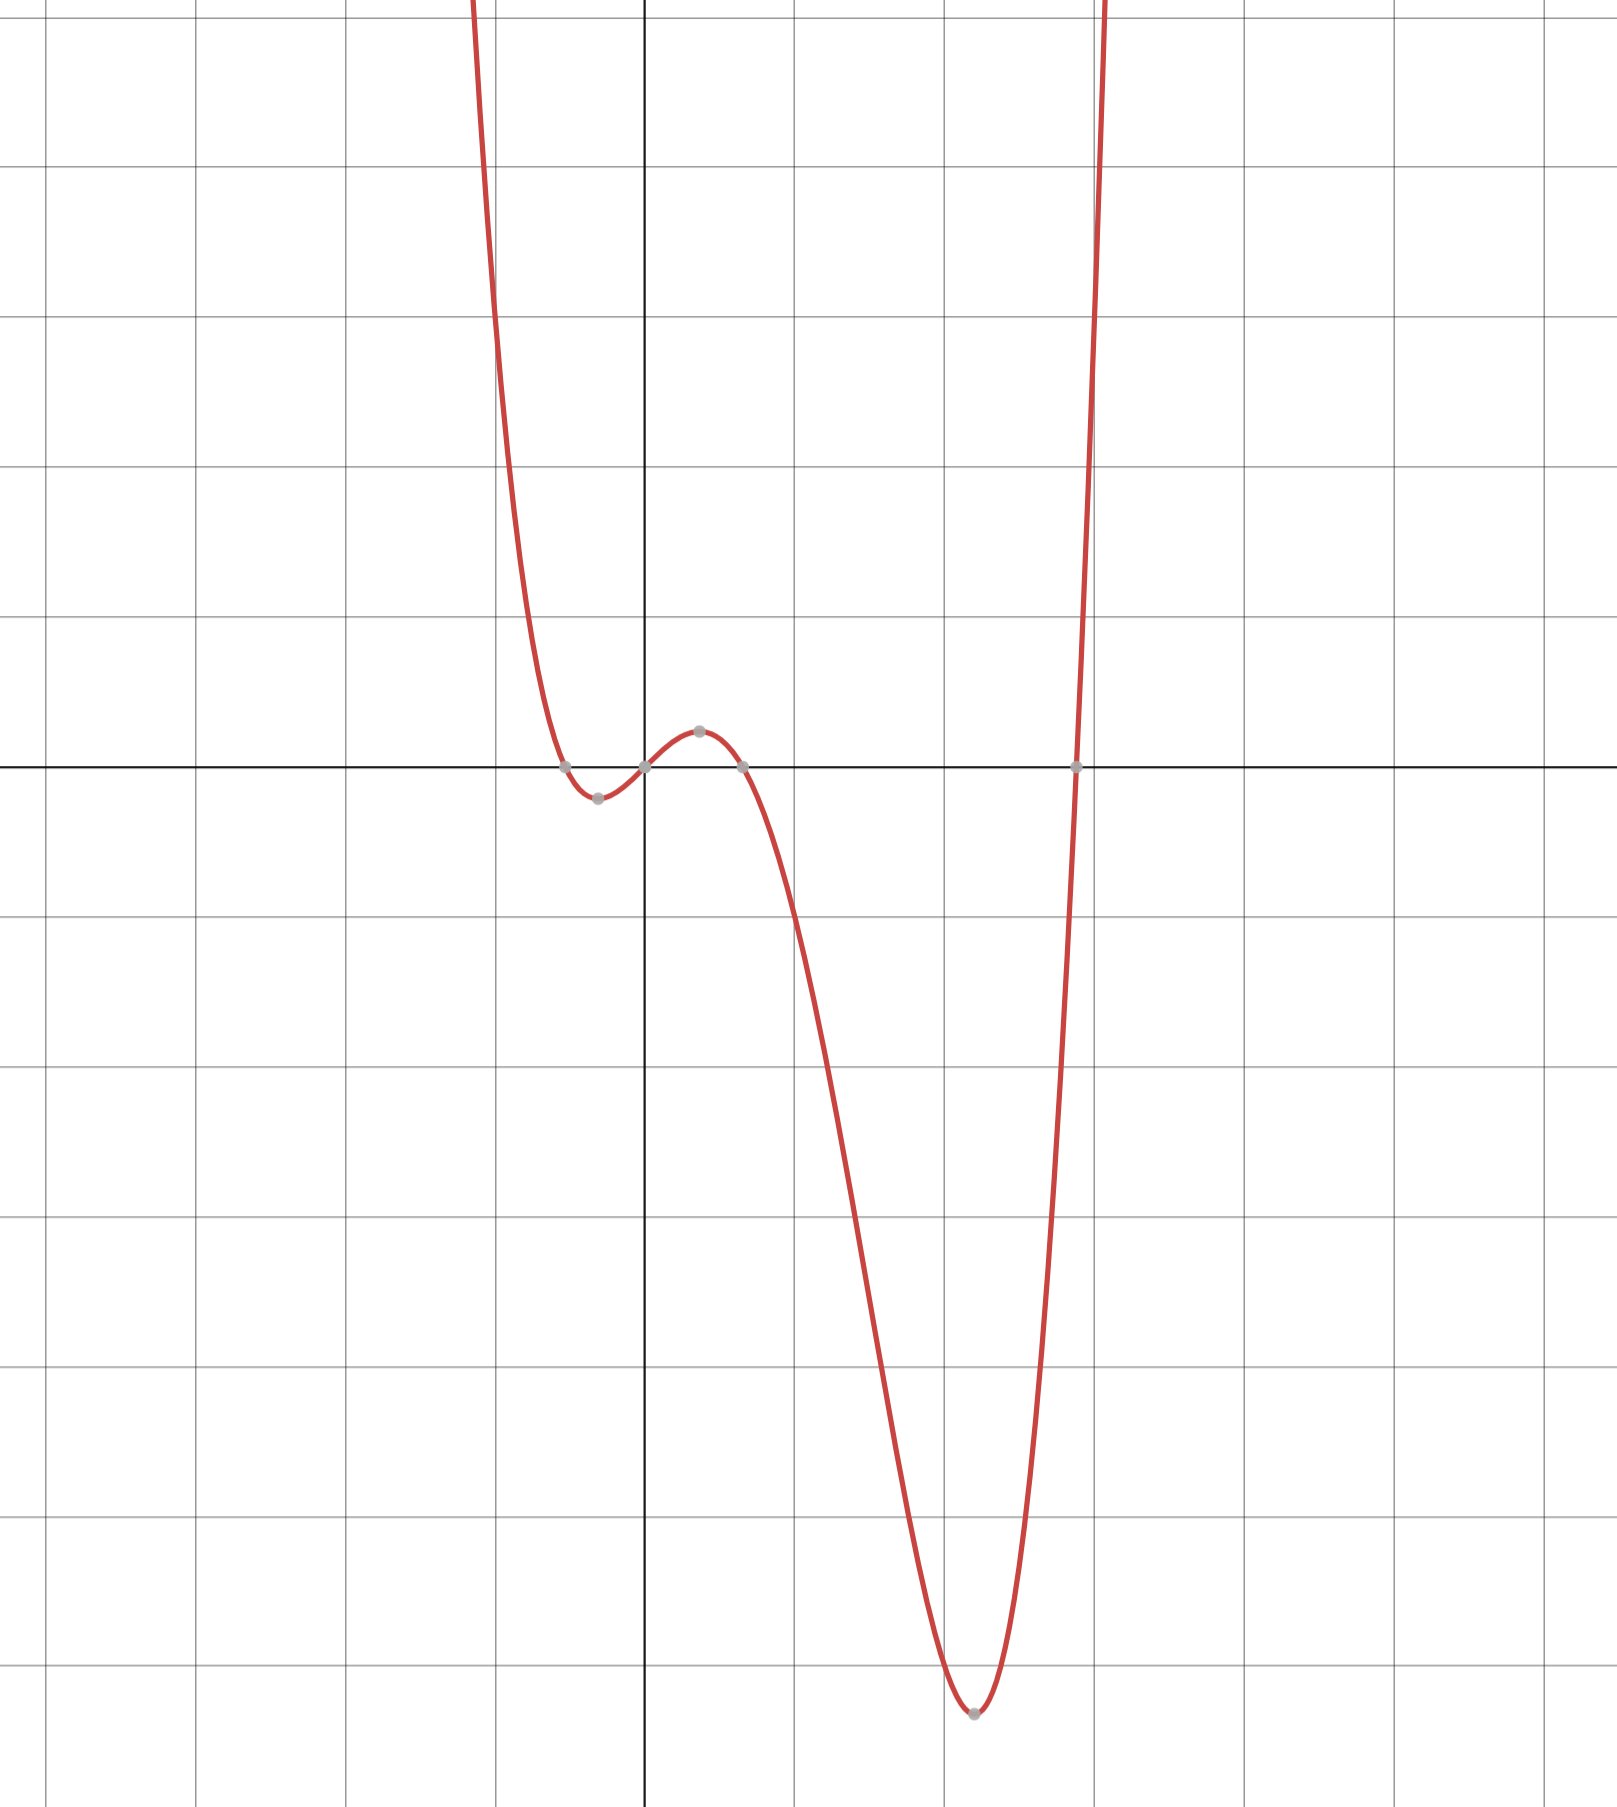
\includegraphics[scale=0.2]{"./fig/case_1.png"}
\end{figure}
\end{example}


\subsection*{Case 2: \( a_n > 0 \) and \(n\) is Odd}


When the leading coefficient \( a_n \) is positive and the degree \( n \) of the polynomial is odd, the graph of the polynomial exhibits the following behavior:

\begin{itemize}
    \item As \( x \to \pm \infty \), the graph tends to \( \pm \infty \).
\end{itemize}


\begin{example}
\(f(x) = x^{5}+3x^{2}-3x\ -1\)
  \begin{itemize}
  \item Degree = 5.
  \item Leadign Coeffecient = 1 $>$ 0.
  \end{itemize}

\begin{figure}[H]
  \centering
  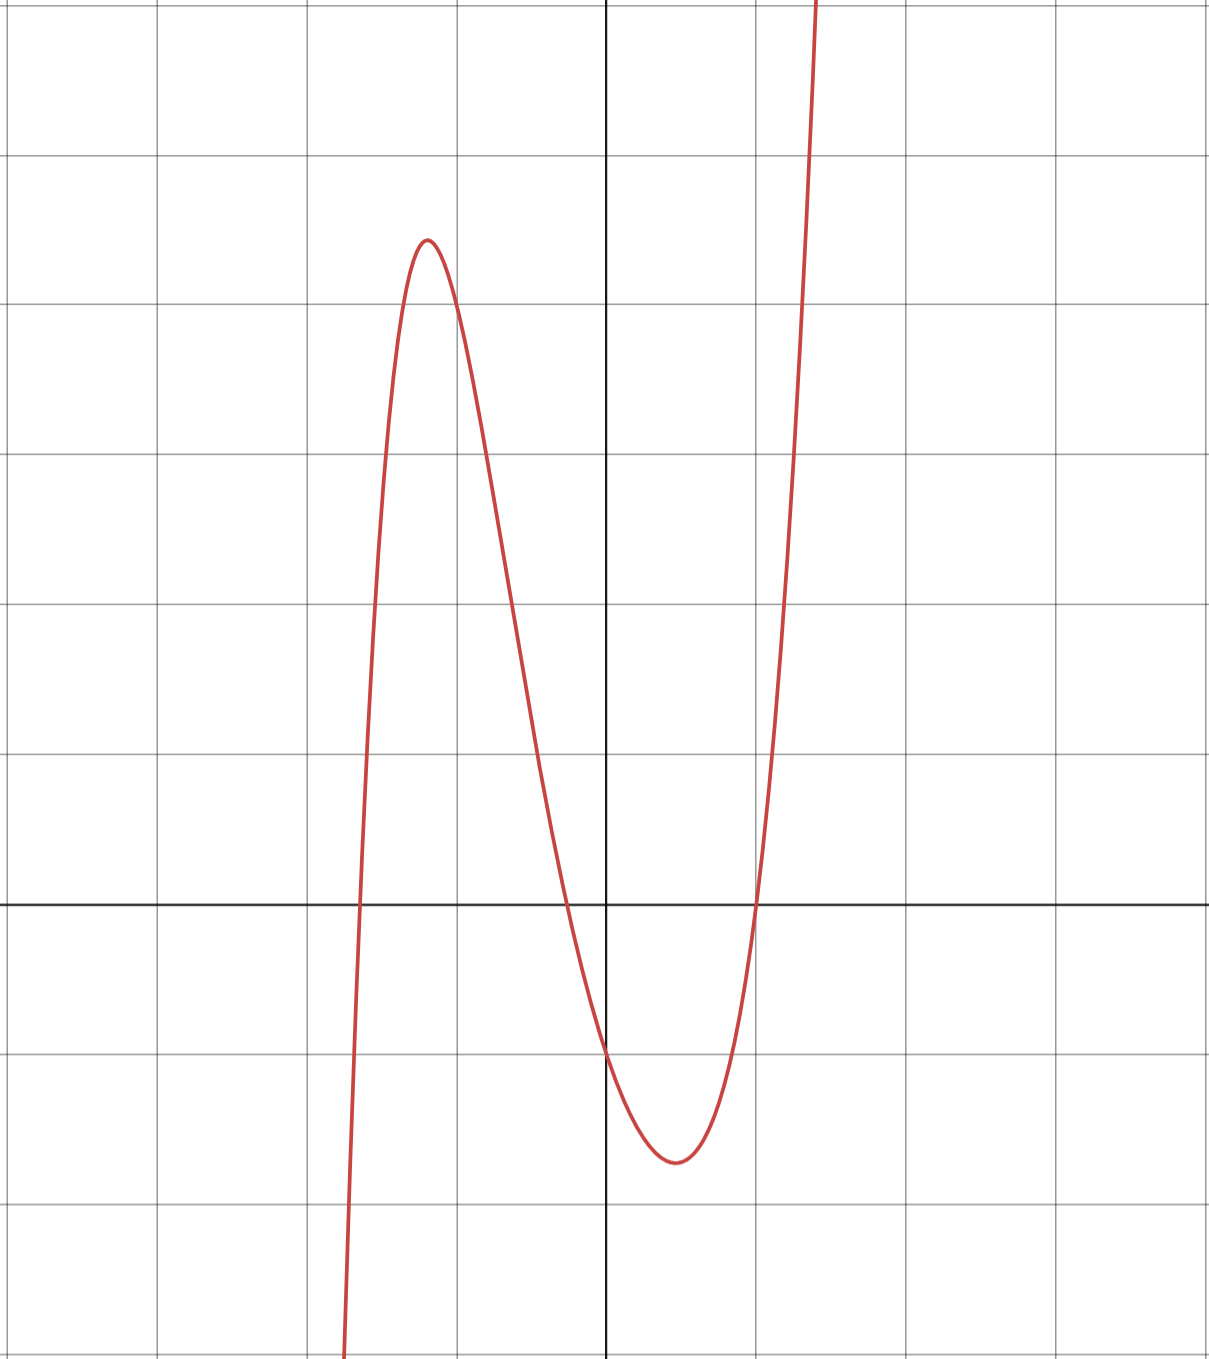
\includegraphics[scale=0.2]{"./fig/case_3.png"}
\end{figure}
\end{example}

\subsection*{Case 3: \( a_n < 0 \) and \(n\) is Even}


When the leading coefficient \( a_n \) is negative and the degree \( n \) of the polynomial is even, the graph of the polynomial exhibits the following behavior:

\begin{itemize}
    \item As \( x \to \pm \infty \), the graph tends to \( - \infty \).
\end{itemize}


\begin{example}
Consider \( f(x) =-1.2x^{4}-3x^{3}+x\)
  Consider   \( f(x) = -2x^6 - 2x^3 + 2 \).
  \begin{itemize}
  \item Degree = 4.
  \item Leadign Coeffecient = -1.2 $<$ 0.
  \end{itemize}


\begin{figure}[H]
  \centering
  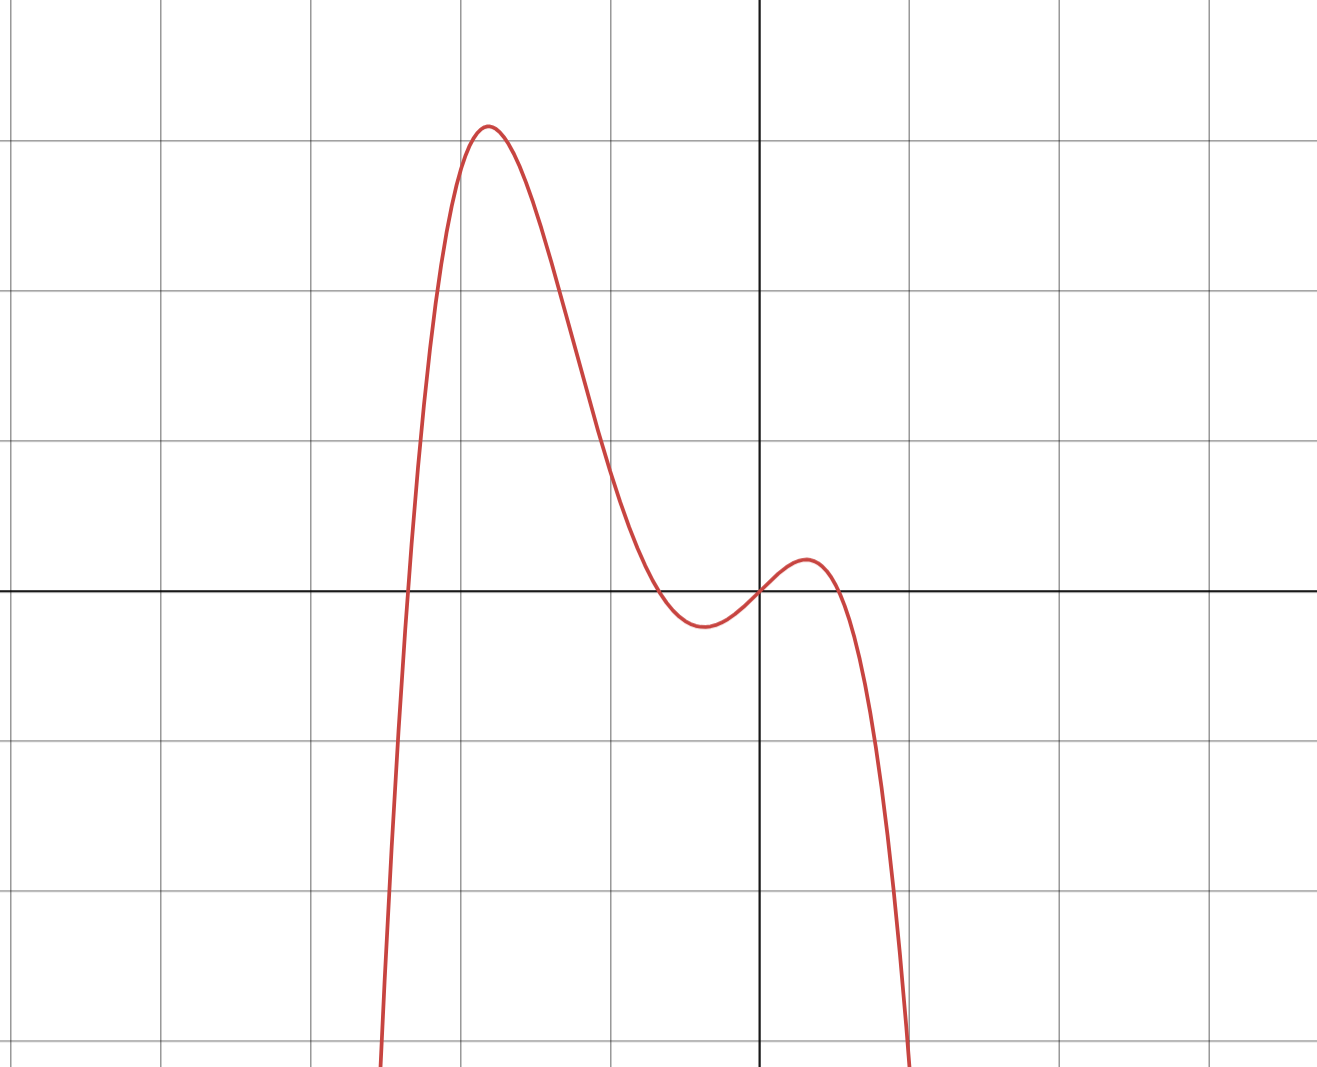
\includegraphics[scale=0.2]{"./fig/case_2.png"}
\end{figure}
\end{example}

\subsection*{Case 4: \( a_n < 0 \) and \(n\) is Odd}

When the leading coefficient \( a_n \) is negative and the degree \( n \) of the polynomial is odd, the graph of the polynomial exhibits the following behavior:

\begin{itemize}
    \item As \( x \to \pm \infty \), the graph tends to \( \mp \infty \).
\end{itemize}


\begin{example}
  Consider   \( f(x) =-3x^{3}+3x^{2\ \ }-2
 \).
  \begin{itemize}
  \item Degree = 6.
  \item Leadign Coeffecient = -1 $<$ 0.
  \end{itemize}

\begin{figure}[H]
  \centering
  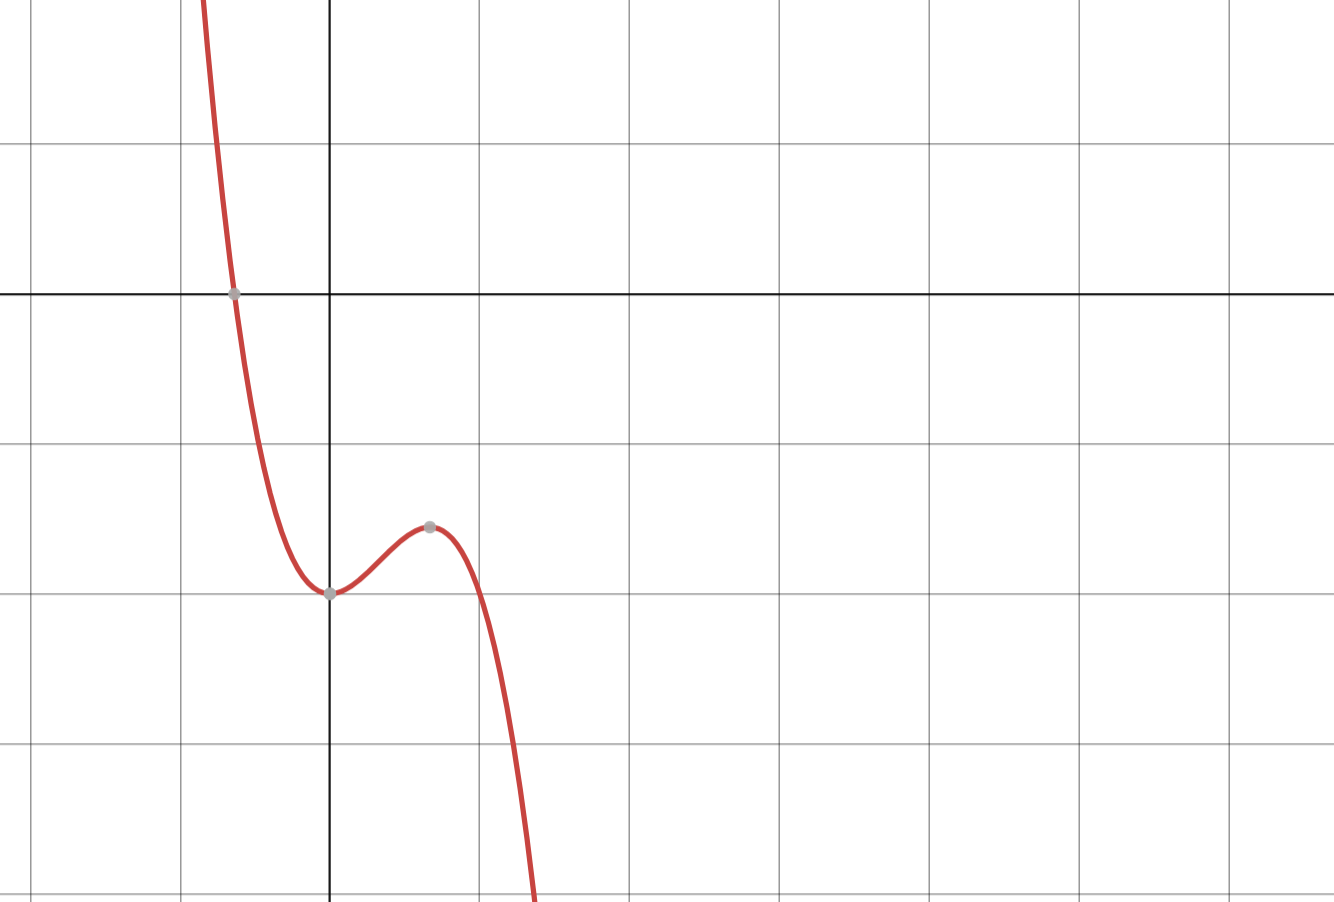
\includegraphics[scale=0.2]{"./fig/case_4.png"}
\end{figure}
\end{example}




- Graph of cubic equations
- Graph of quartic equations
- Find the degree and leading coefficient of a polynomial by looking at its graph
- Horizontal and vertical asymptotes
\section{Rational Functions}
\begin{definition}[Rational Functions]
A rational function is a function that can be expressed as the ratio of two polynomials, i.e.,
\[
f(x) = \frac{P(x)}{Q(x)}
\]
where \( P(x) \) and \( Q(x) \) are polynomials and \( Q(x) \neq 0 \). 
\end{definition}
The behavior of a rational function is often analyzed using asymptotes, which are lines that the graph of the function approaches but never touches.

There are two main types of asymptotes: vertical asymptotes and horizontal asymptotes.


\subsection*{Vertical Asymptotes}

A vertical asymptote occurs when the function approaches infinity or negative infinity as \( x \) approaches a certain value from the left or right.

These asymptotes are generally found by determining where the denominator of the rational function equals zero, provided that the numerator does not also equal zero at the same value.

Steps to Find Vertical Asymptotes:
\begin{itemize}
\item Set the denominator \( Q(x) = 0 \) and solve for \( x \).
\item If the numerator \( P(x) \) does not equal zero at the same values of \( x \), then those values are vertical asymptotes.
\end{itemize}

\begin{example}
Find the Vertical Asymptotes of \( f(x) = \frac{1}{x^2 - 4} \)

\begin{figure}[H]
  \centering
  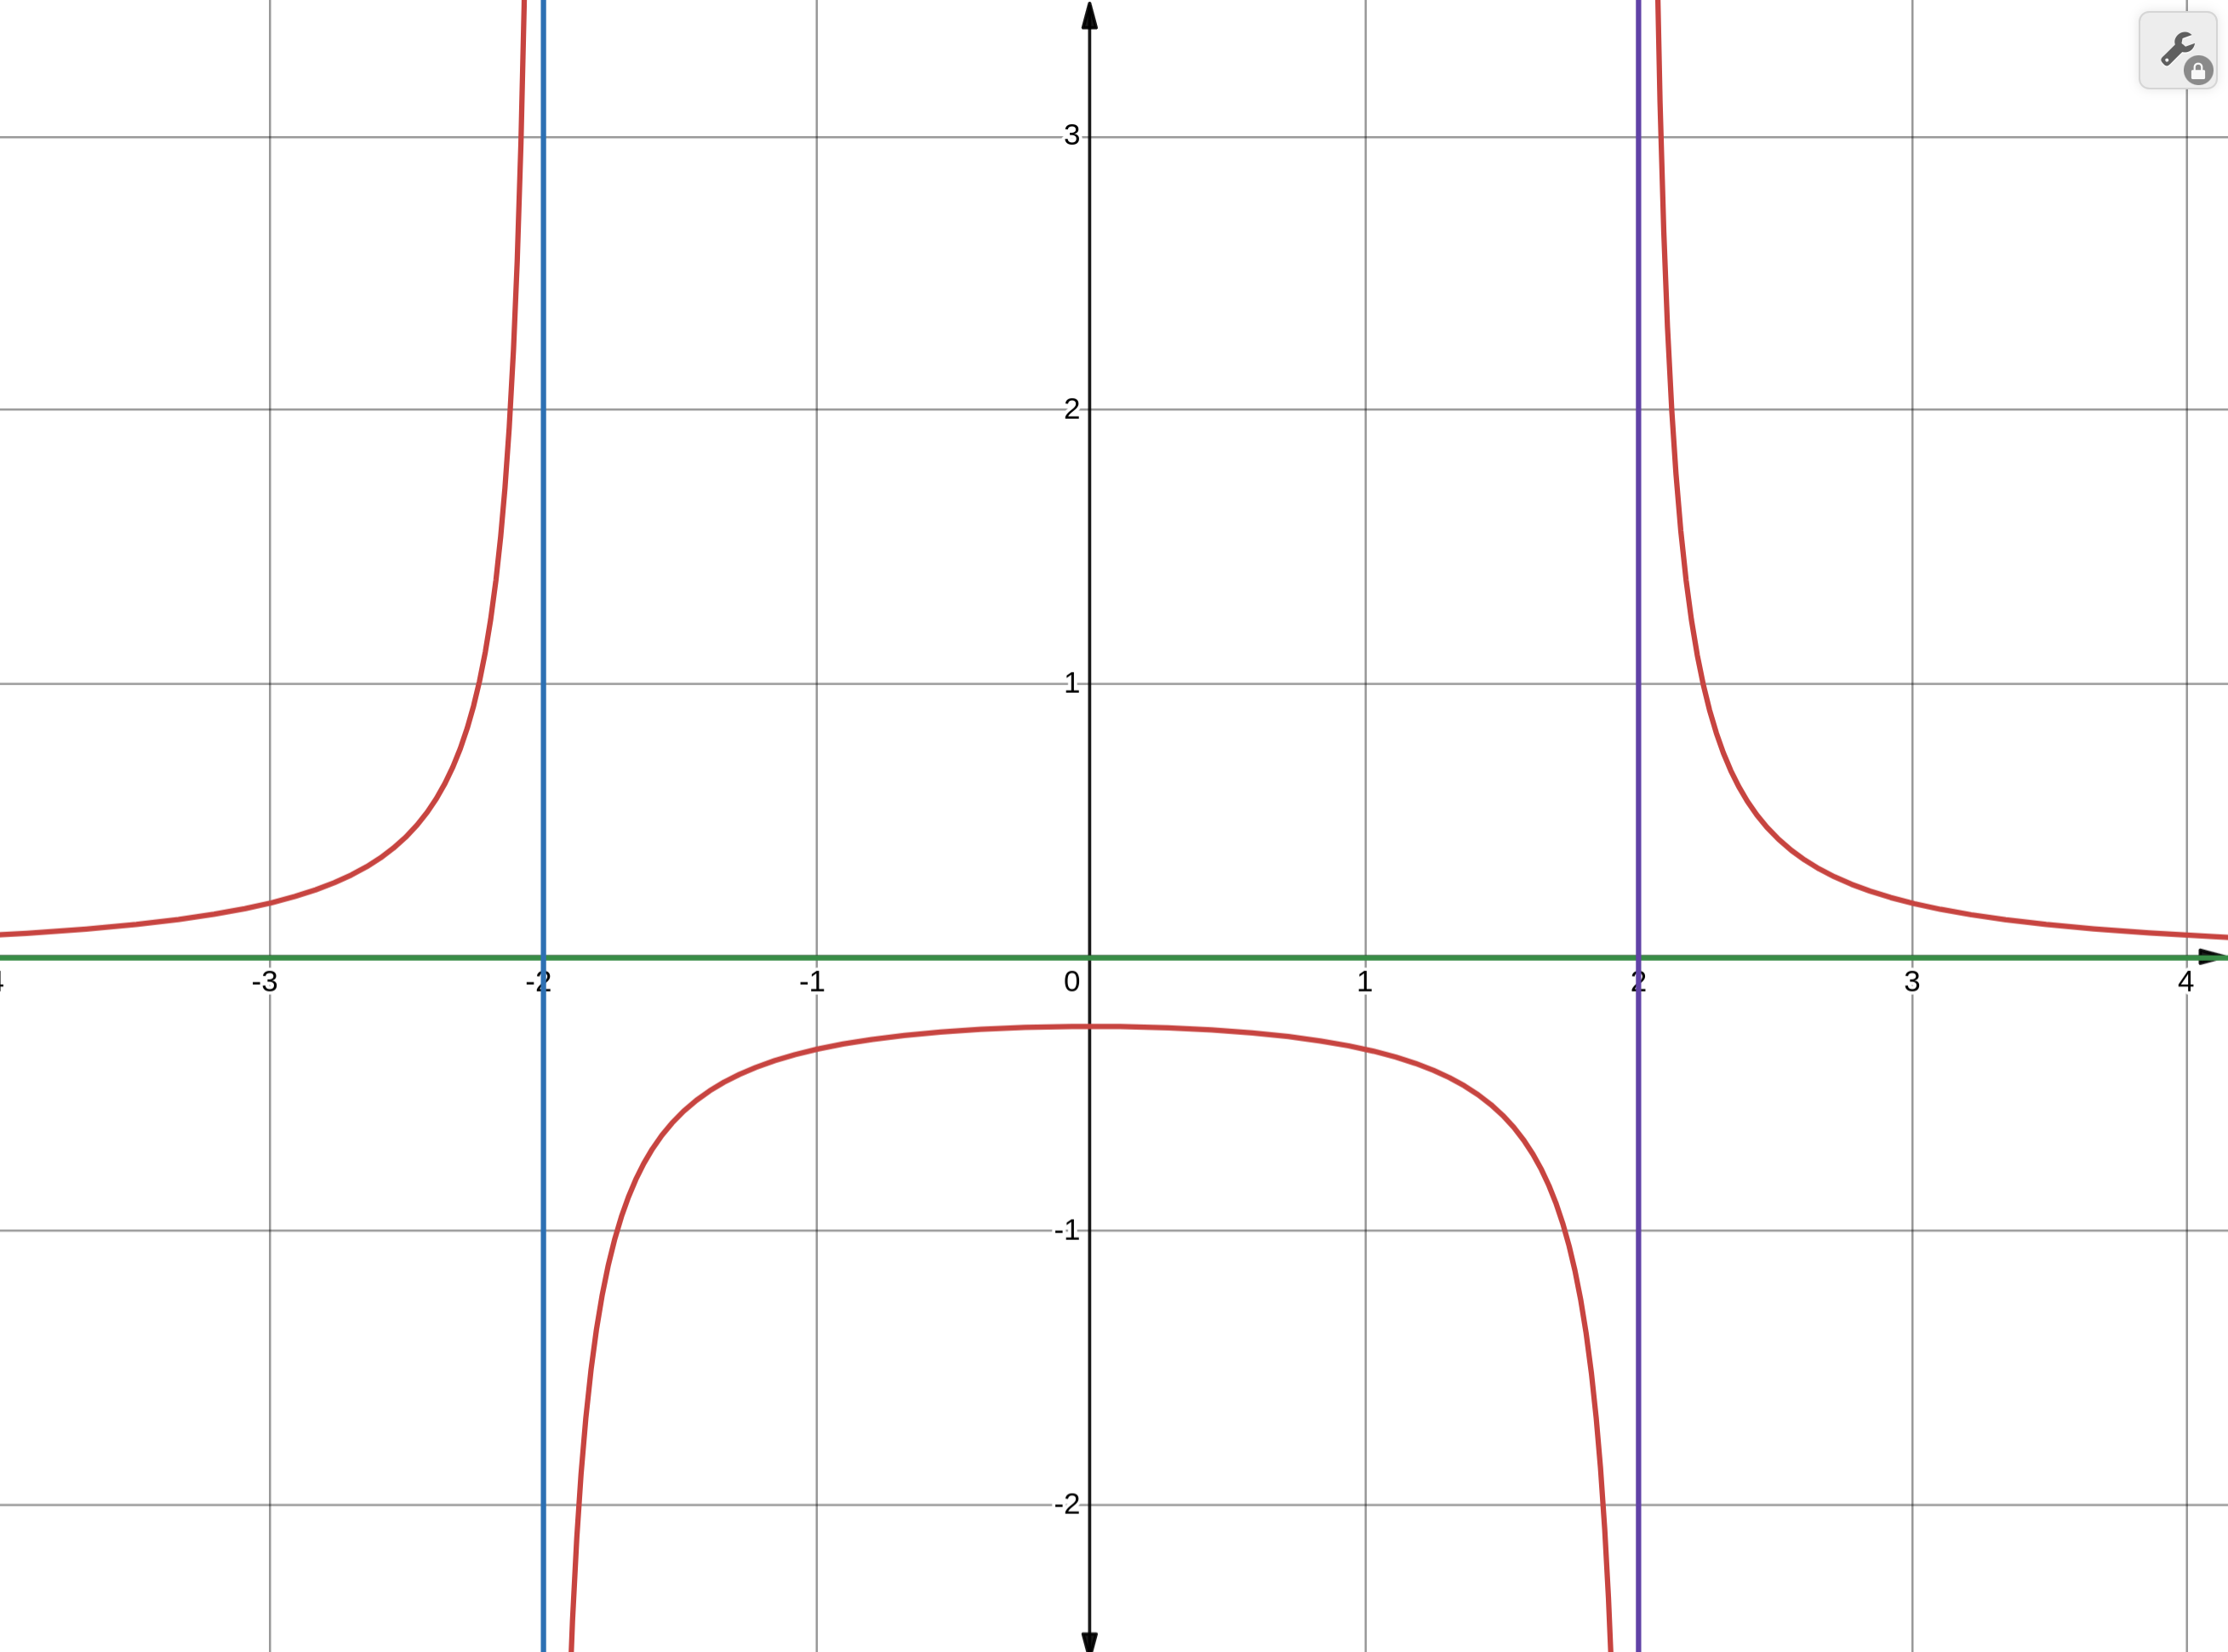
\includegraphics[scale=0.2]{"./fig/vert_asym.png"}
\end{figure}
\end{example}

Consider the rational function

\[
f(x) = \frac{1}{x^2 - 4}
\]

To find the vertical asymptotes, we set the denominator equal to zero:

\[
x^2 - 4 = 0.
\]

Solving this equation, we get

\[
x^2 = 4 \quad \Rightarrow \quad x = \pm 2.
\]

Since the numerator is not zero at \( x = 2 \) or \( x = -2 \), the vertical asymptotes of this function are at

\[
x = 2 \quad \text{and} \quad x = -2
\]

Thus, the graph of \( f(x) \) has vertical asymptotes at \( x = 2 \) and \( x = -2 \).

\subsection*{Horizontal Asymptotes}

A horizontal asymptote describes the behavior of a rational function as \( x \to \infty \) or \( x \to -\infty \).

The horizontal asymptote indicates the value that the function approaches as \( x \) becomes very large or very small.

Steps to Find Horizontal Asymptotes:

\begin{itemize}
    \item If \( \deg(P(x)) < \deg(Q(x)) \), then the horizontal asymptote is \( y = 0 \).
    \item If \( \deg(P(x)) = \deg(Q(x)) \), then the horizontal asymptote is \( y = \frac{\text{leading coefficient of } P(x)}{\text{leading coefficient of } Q(x)} \).
    \item If \( \deg(P(x)) > \deg(Q(x)) \), there is no horizontal asymptote (but there might be an oblique/slant asymptote).
\end{itemize}

\begin{example}
Find the Horizontal Asymptote of \( f(x) = \frac{3x^2 + 5}{2x^2 + 7} \)
\end{example}

\textbf{Solution}

Here, both the numerator and the denominator are of degree 2. Therefore, we apply the second rule:

\[
y = \frac{\text{leading coefficient of } P(x)}{\text{leading coefficient of } Q(x)} = \frac{3}{2}
\]

Thus, the horizontal asymptote of the function is:

\[
y = \frac{3}{2}
\]


\begin{figure}[H]
  \centering
  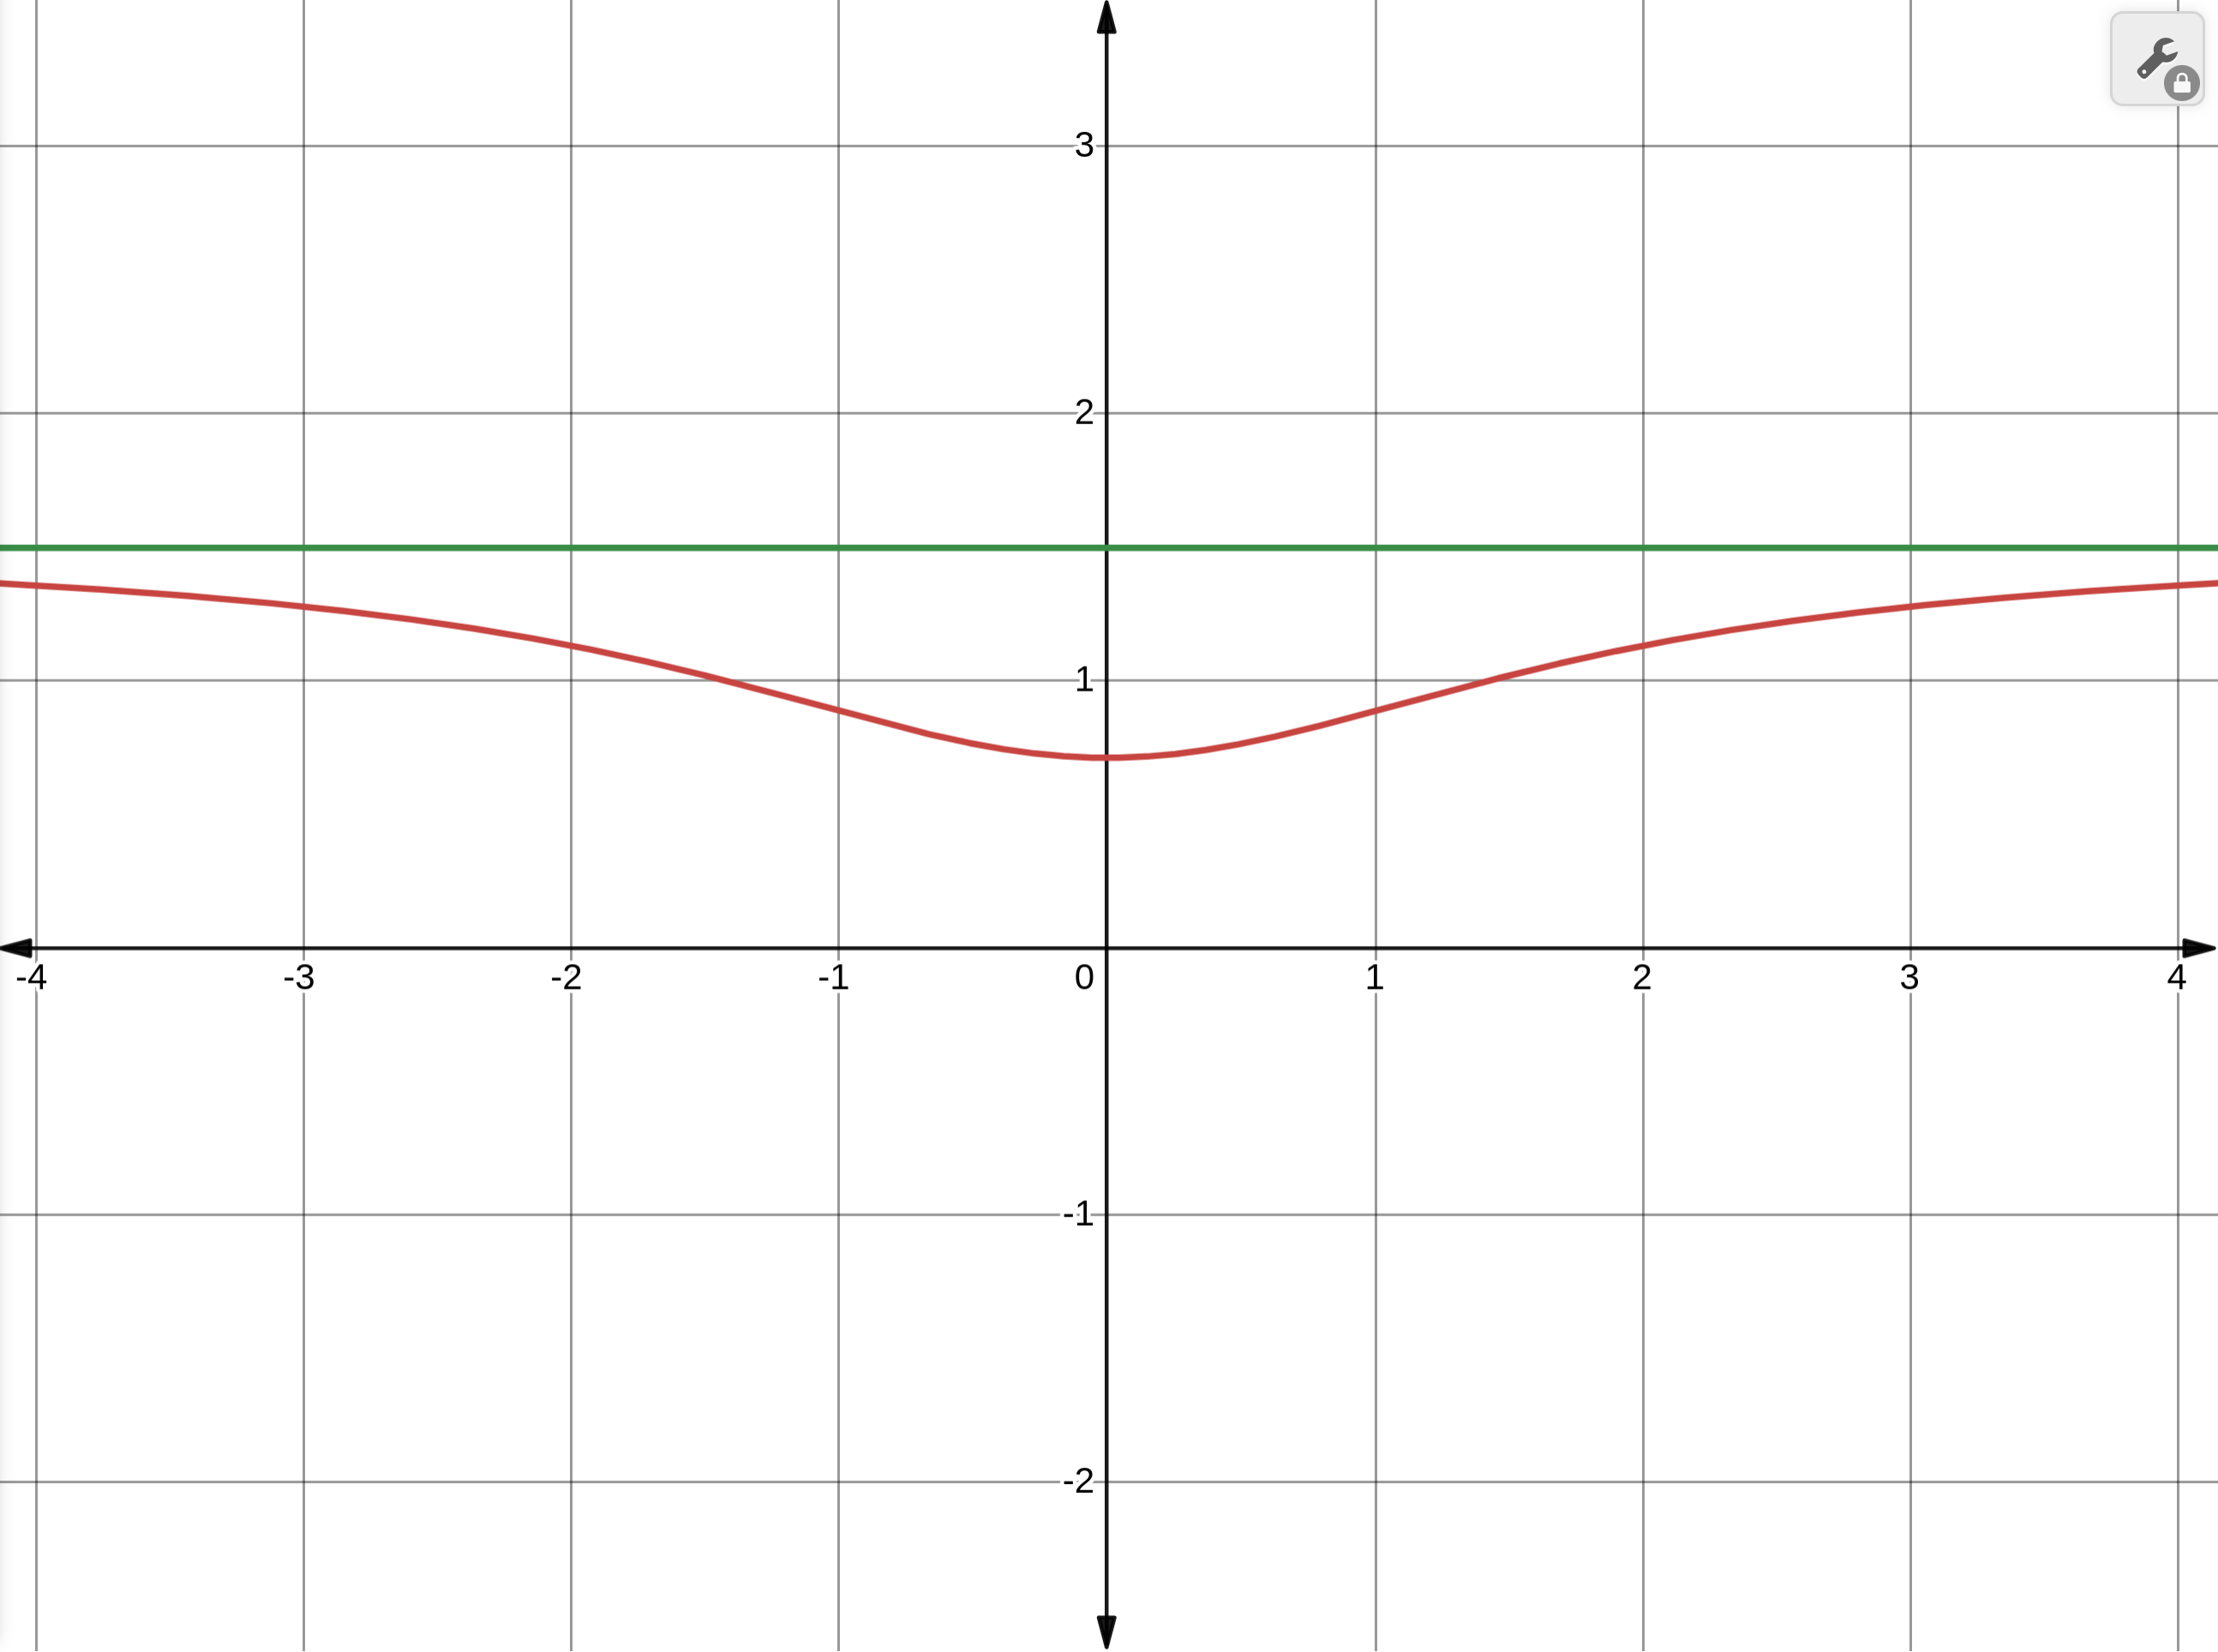
\includegraphics[scale=0.2]{"./fig/ho_asym1.png"}
\end{figure}

\begin{example}
Find the Horizontal Asymptote of \( f\left(x\right)\ =\ \frac{3x-2}{2x^{2}+7}\)



\begin{figure}[H]
  \centering
  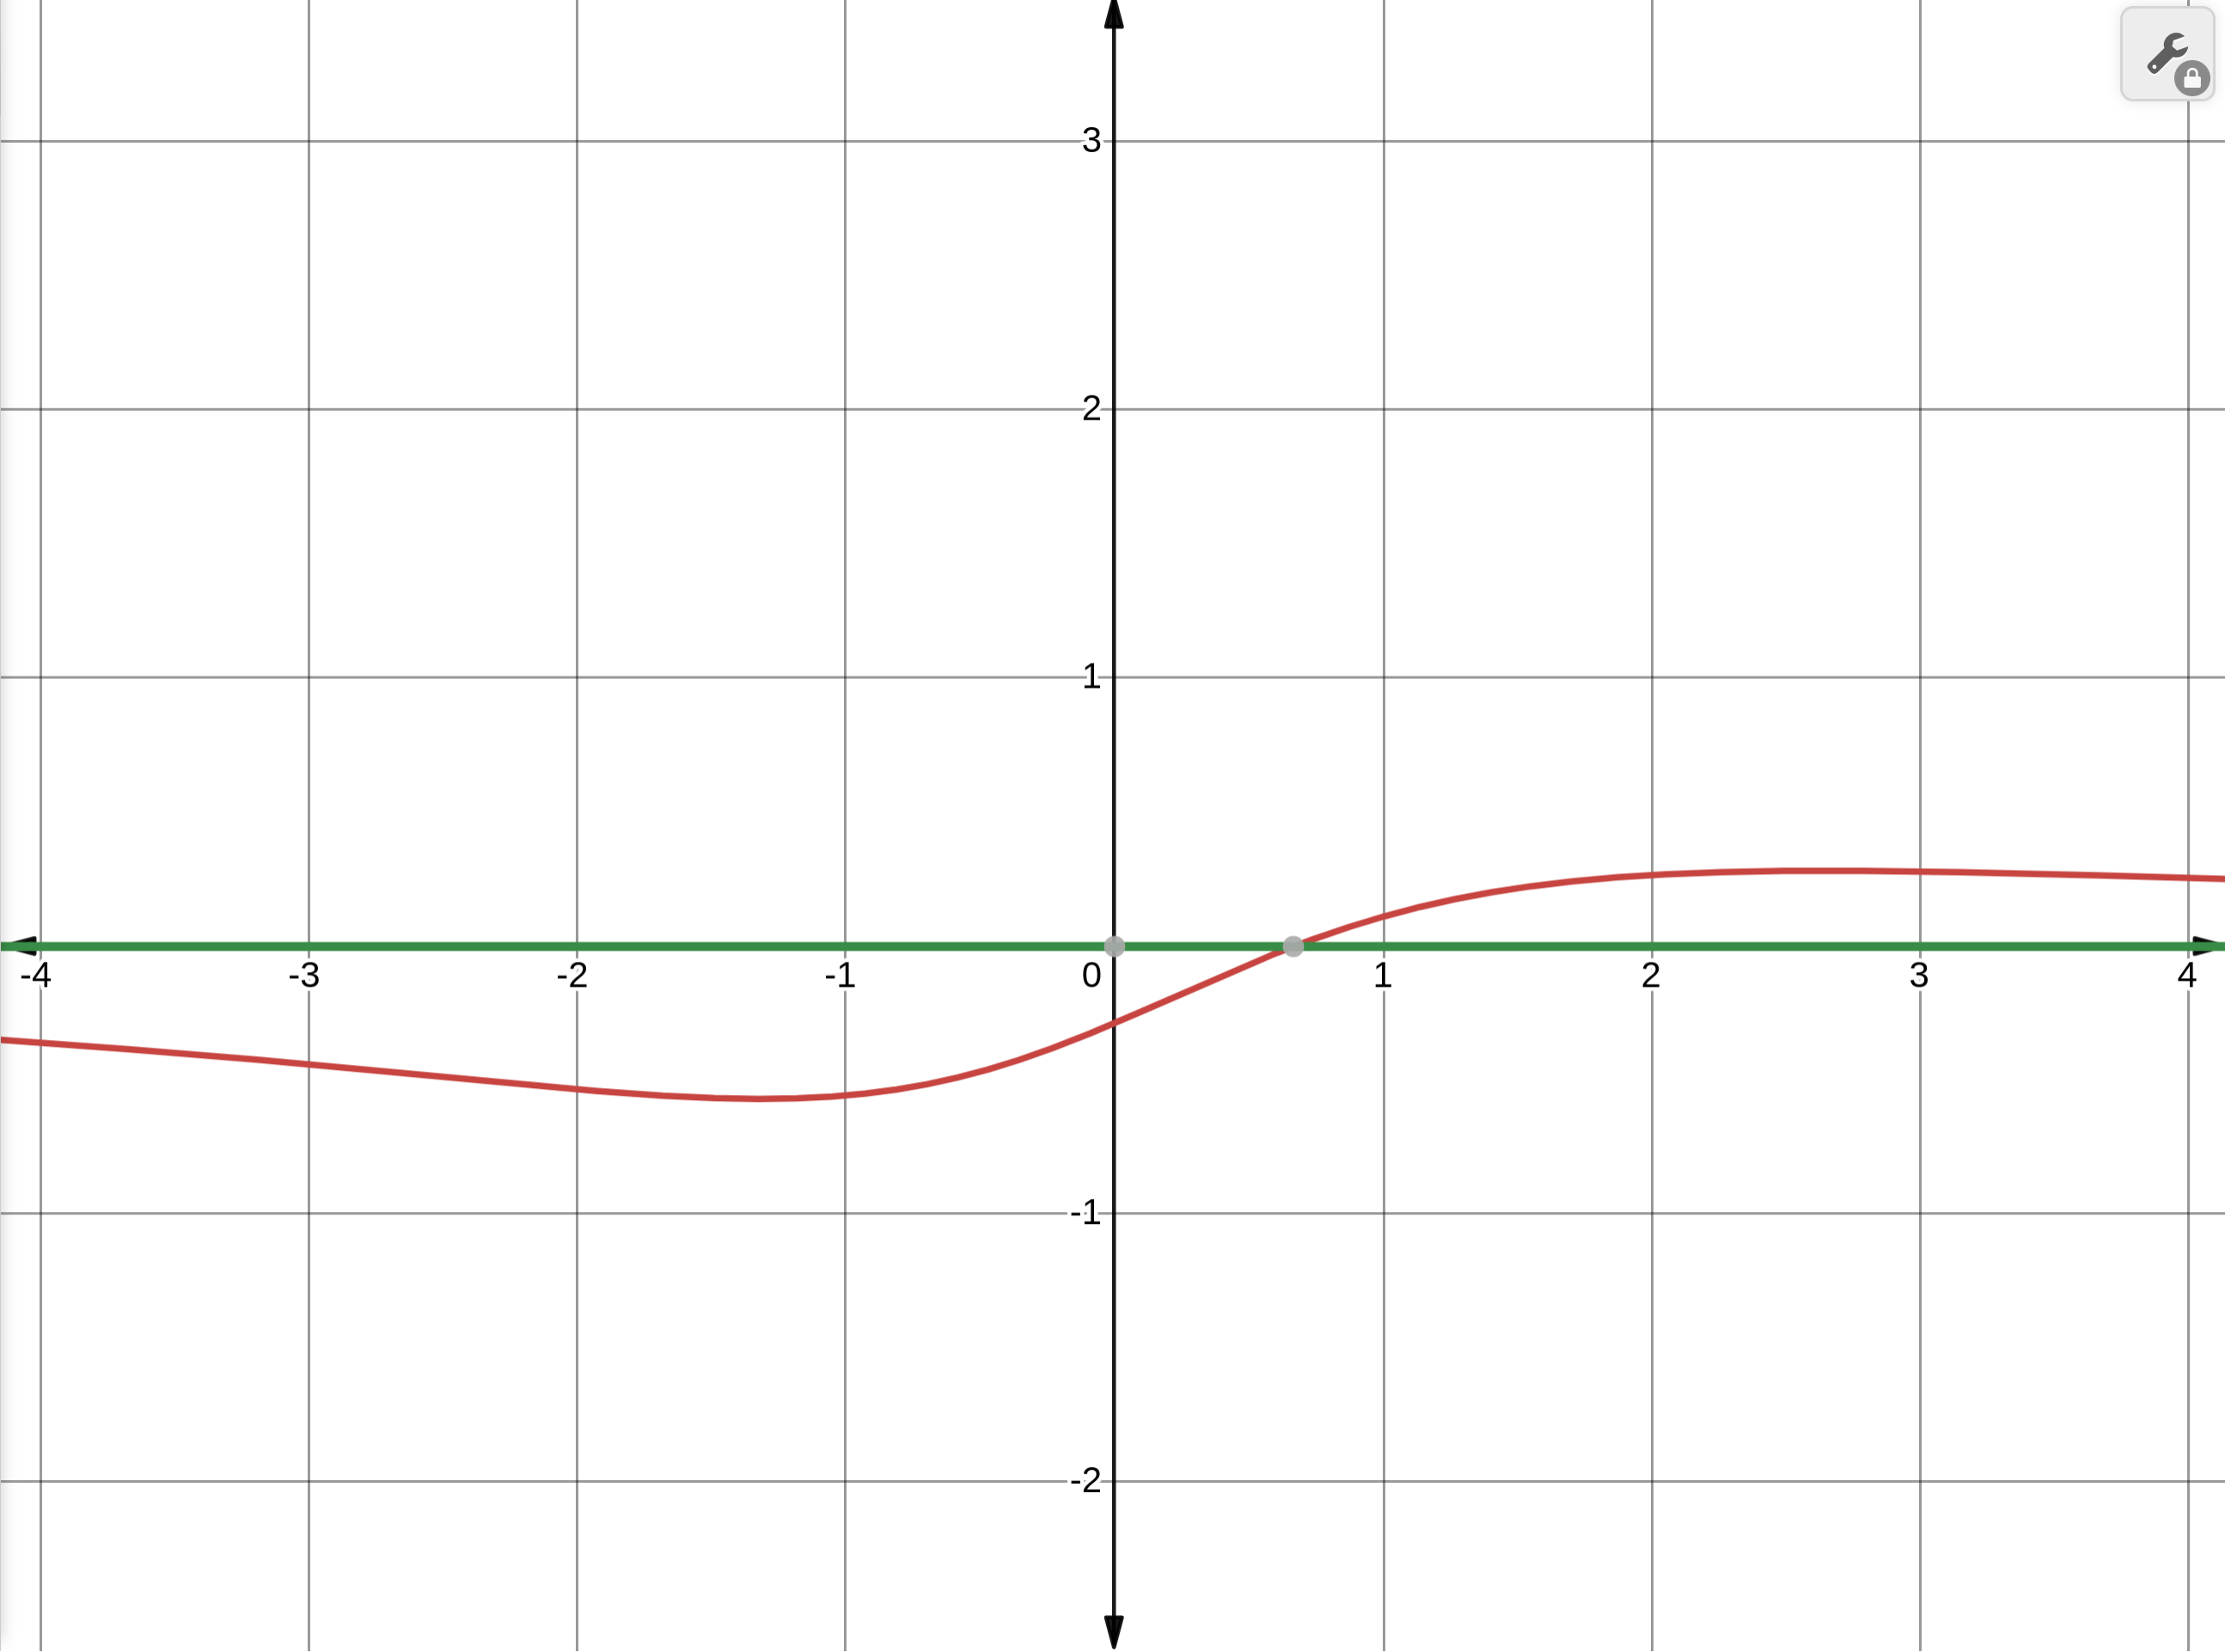
\includegraphics[scale=0.2]{"./fig/ho_asym2.png"}
\end{figure}

\end{example}
\begin{example}
Find the Horizontal Asymptote of \( f(x) = \frac{x^3 - 4x}{x^2 + 1} \)
\end{example}

\textbf{Solution:}

Here, the degree of the numerator is 3 and the degree of the denominator is 2. Since \( \deg(P(x)) > \deg(Q(x)) \), there is no horizontal asymptote. Instead, there may be an oblique or slant asymptote.

\begin{figure}[H]
  \centering
  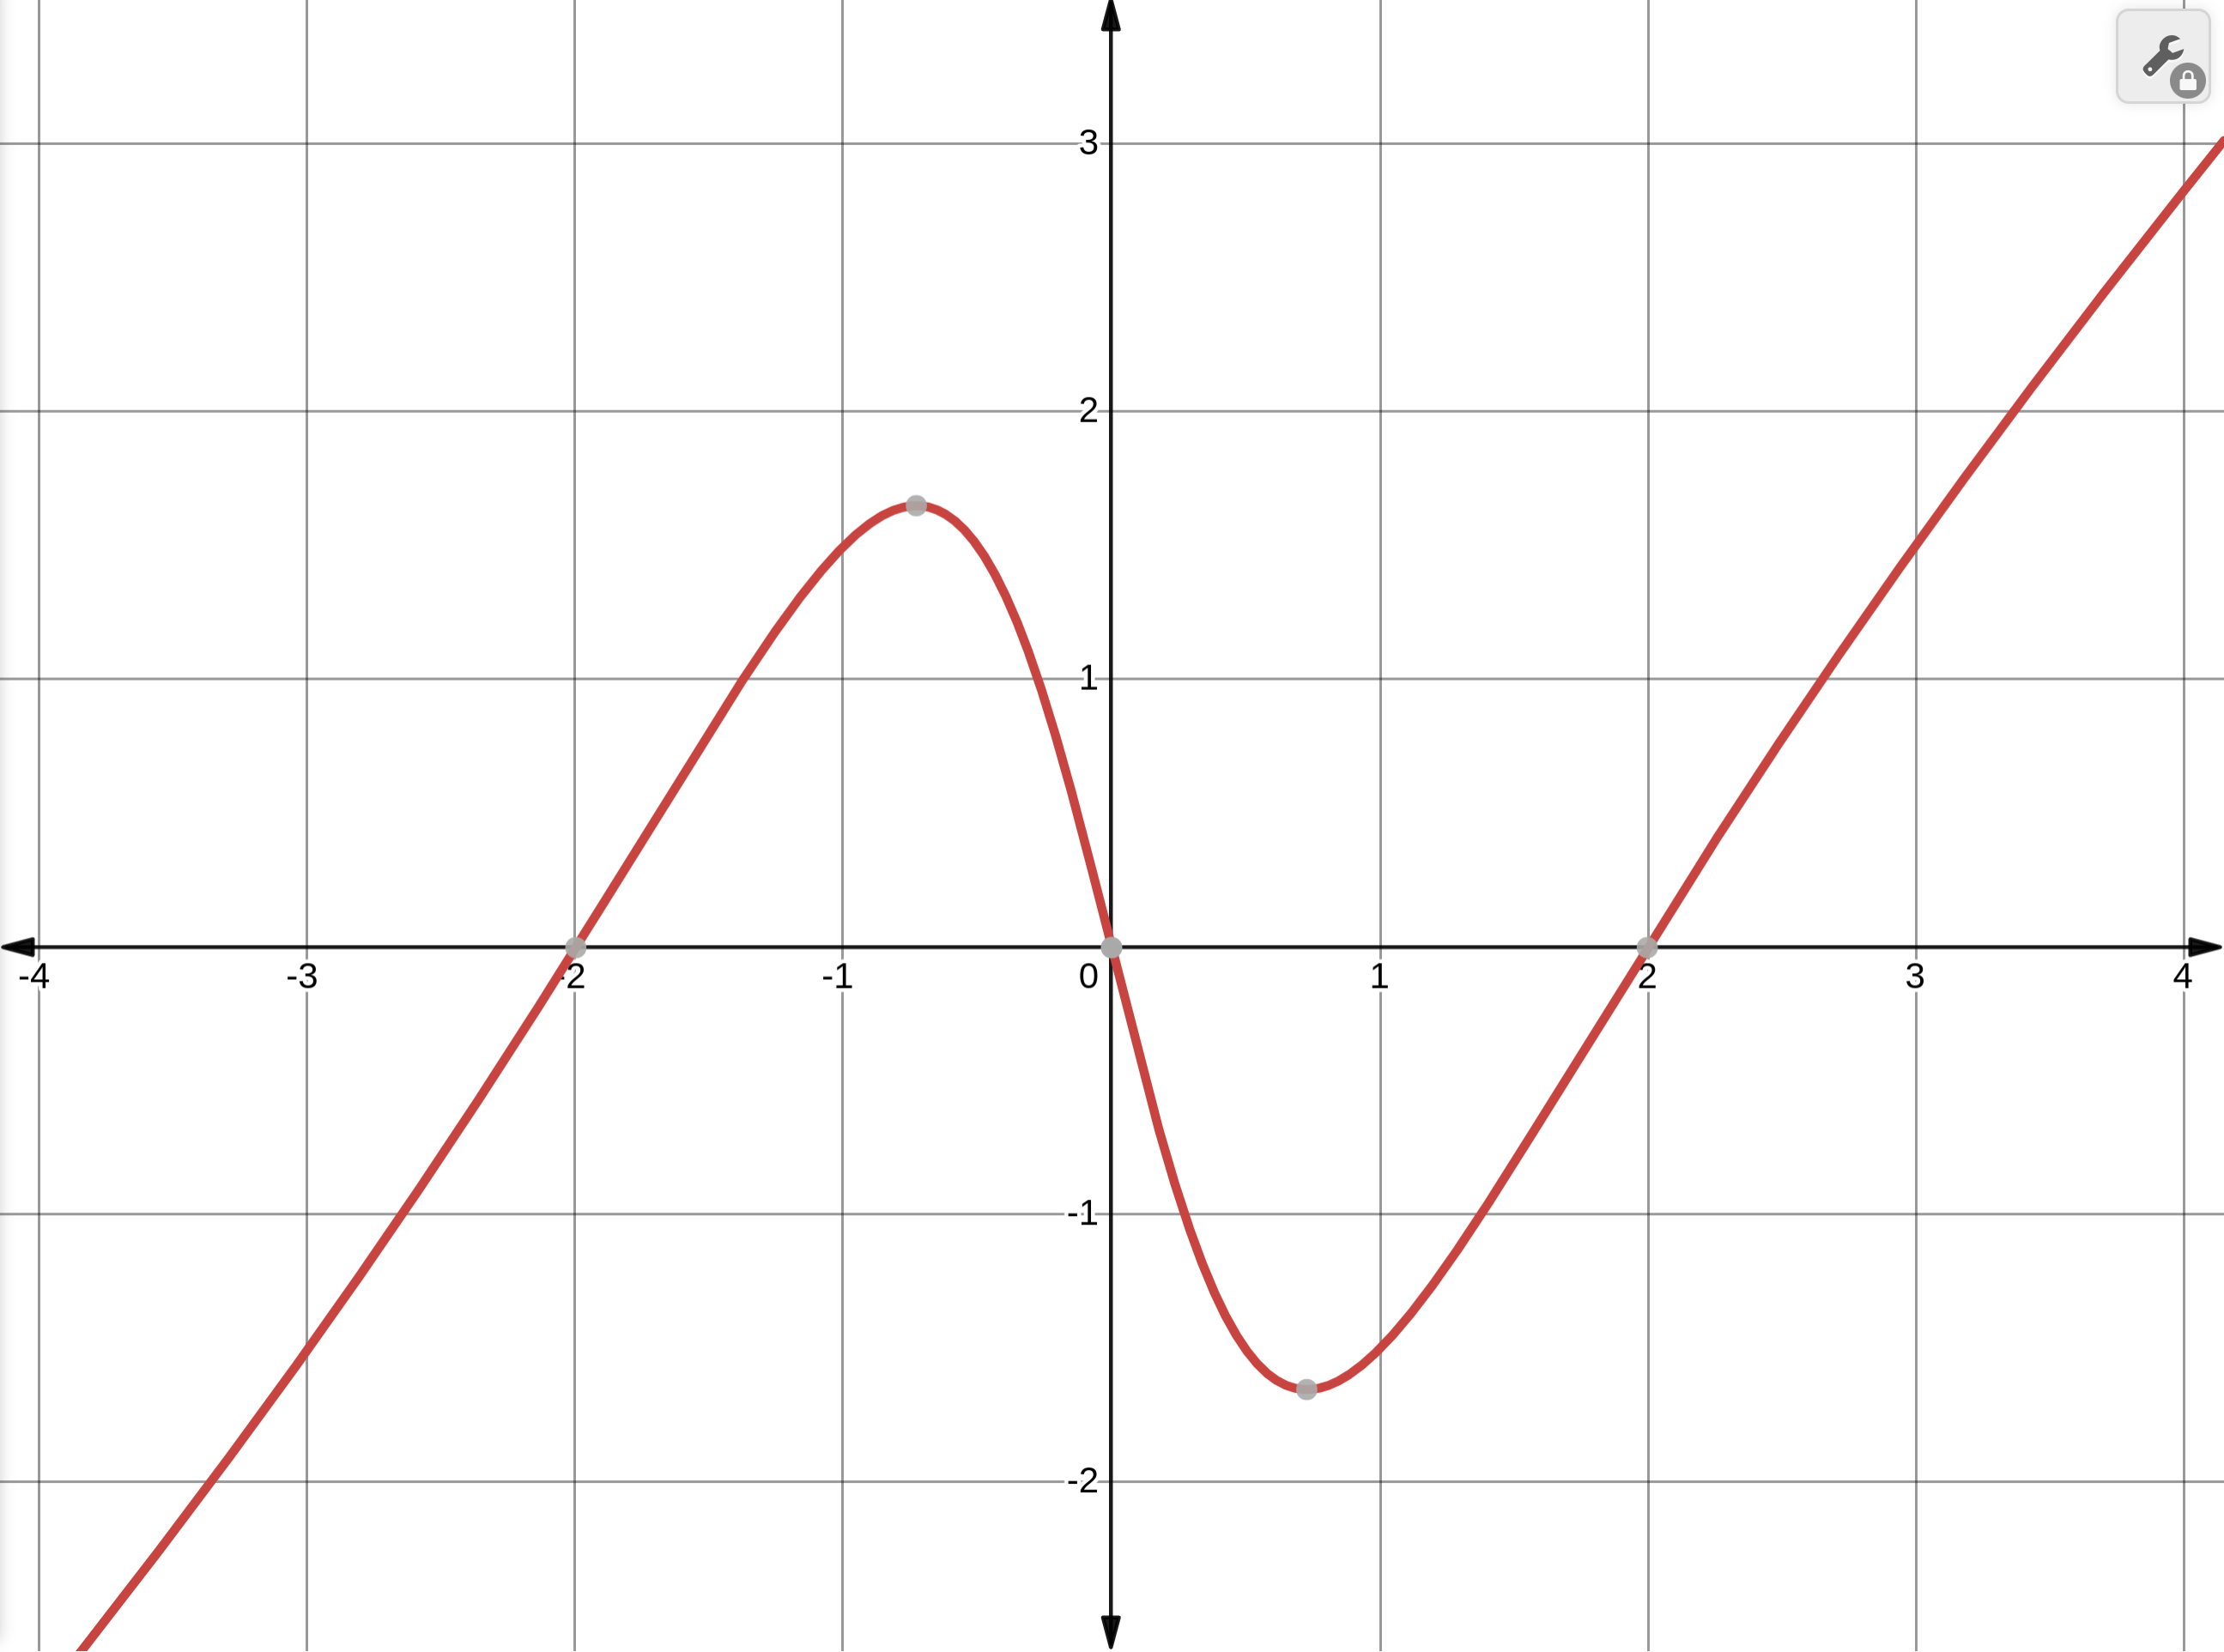
\includegraphics[scale=0.2]{"./fig/ho_asym3.png"}
\end{figure}
\section{Exponential Functions}

\begin{definition}
[Exponential Function]
An exponential function is generally given by:
\[
f(x) = a^x
\]
where \( a \neq 1 \) \( a>0 \). 
\end{definition}

The overall behavior of plot of $f(x)$ depends whether $0<a<1$ or $a>1$.

\subsection*{Graph of \(a^{x}\) when \(a<0\)}
\begin{figure}[H]
  \centering
  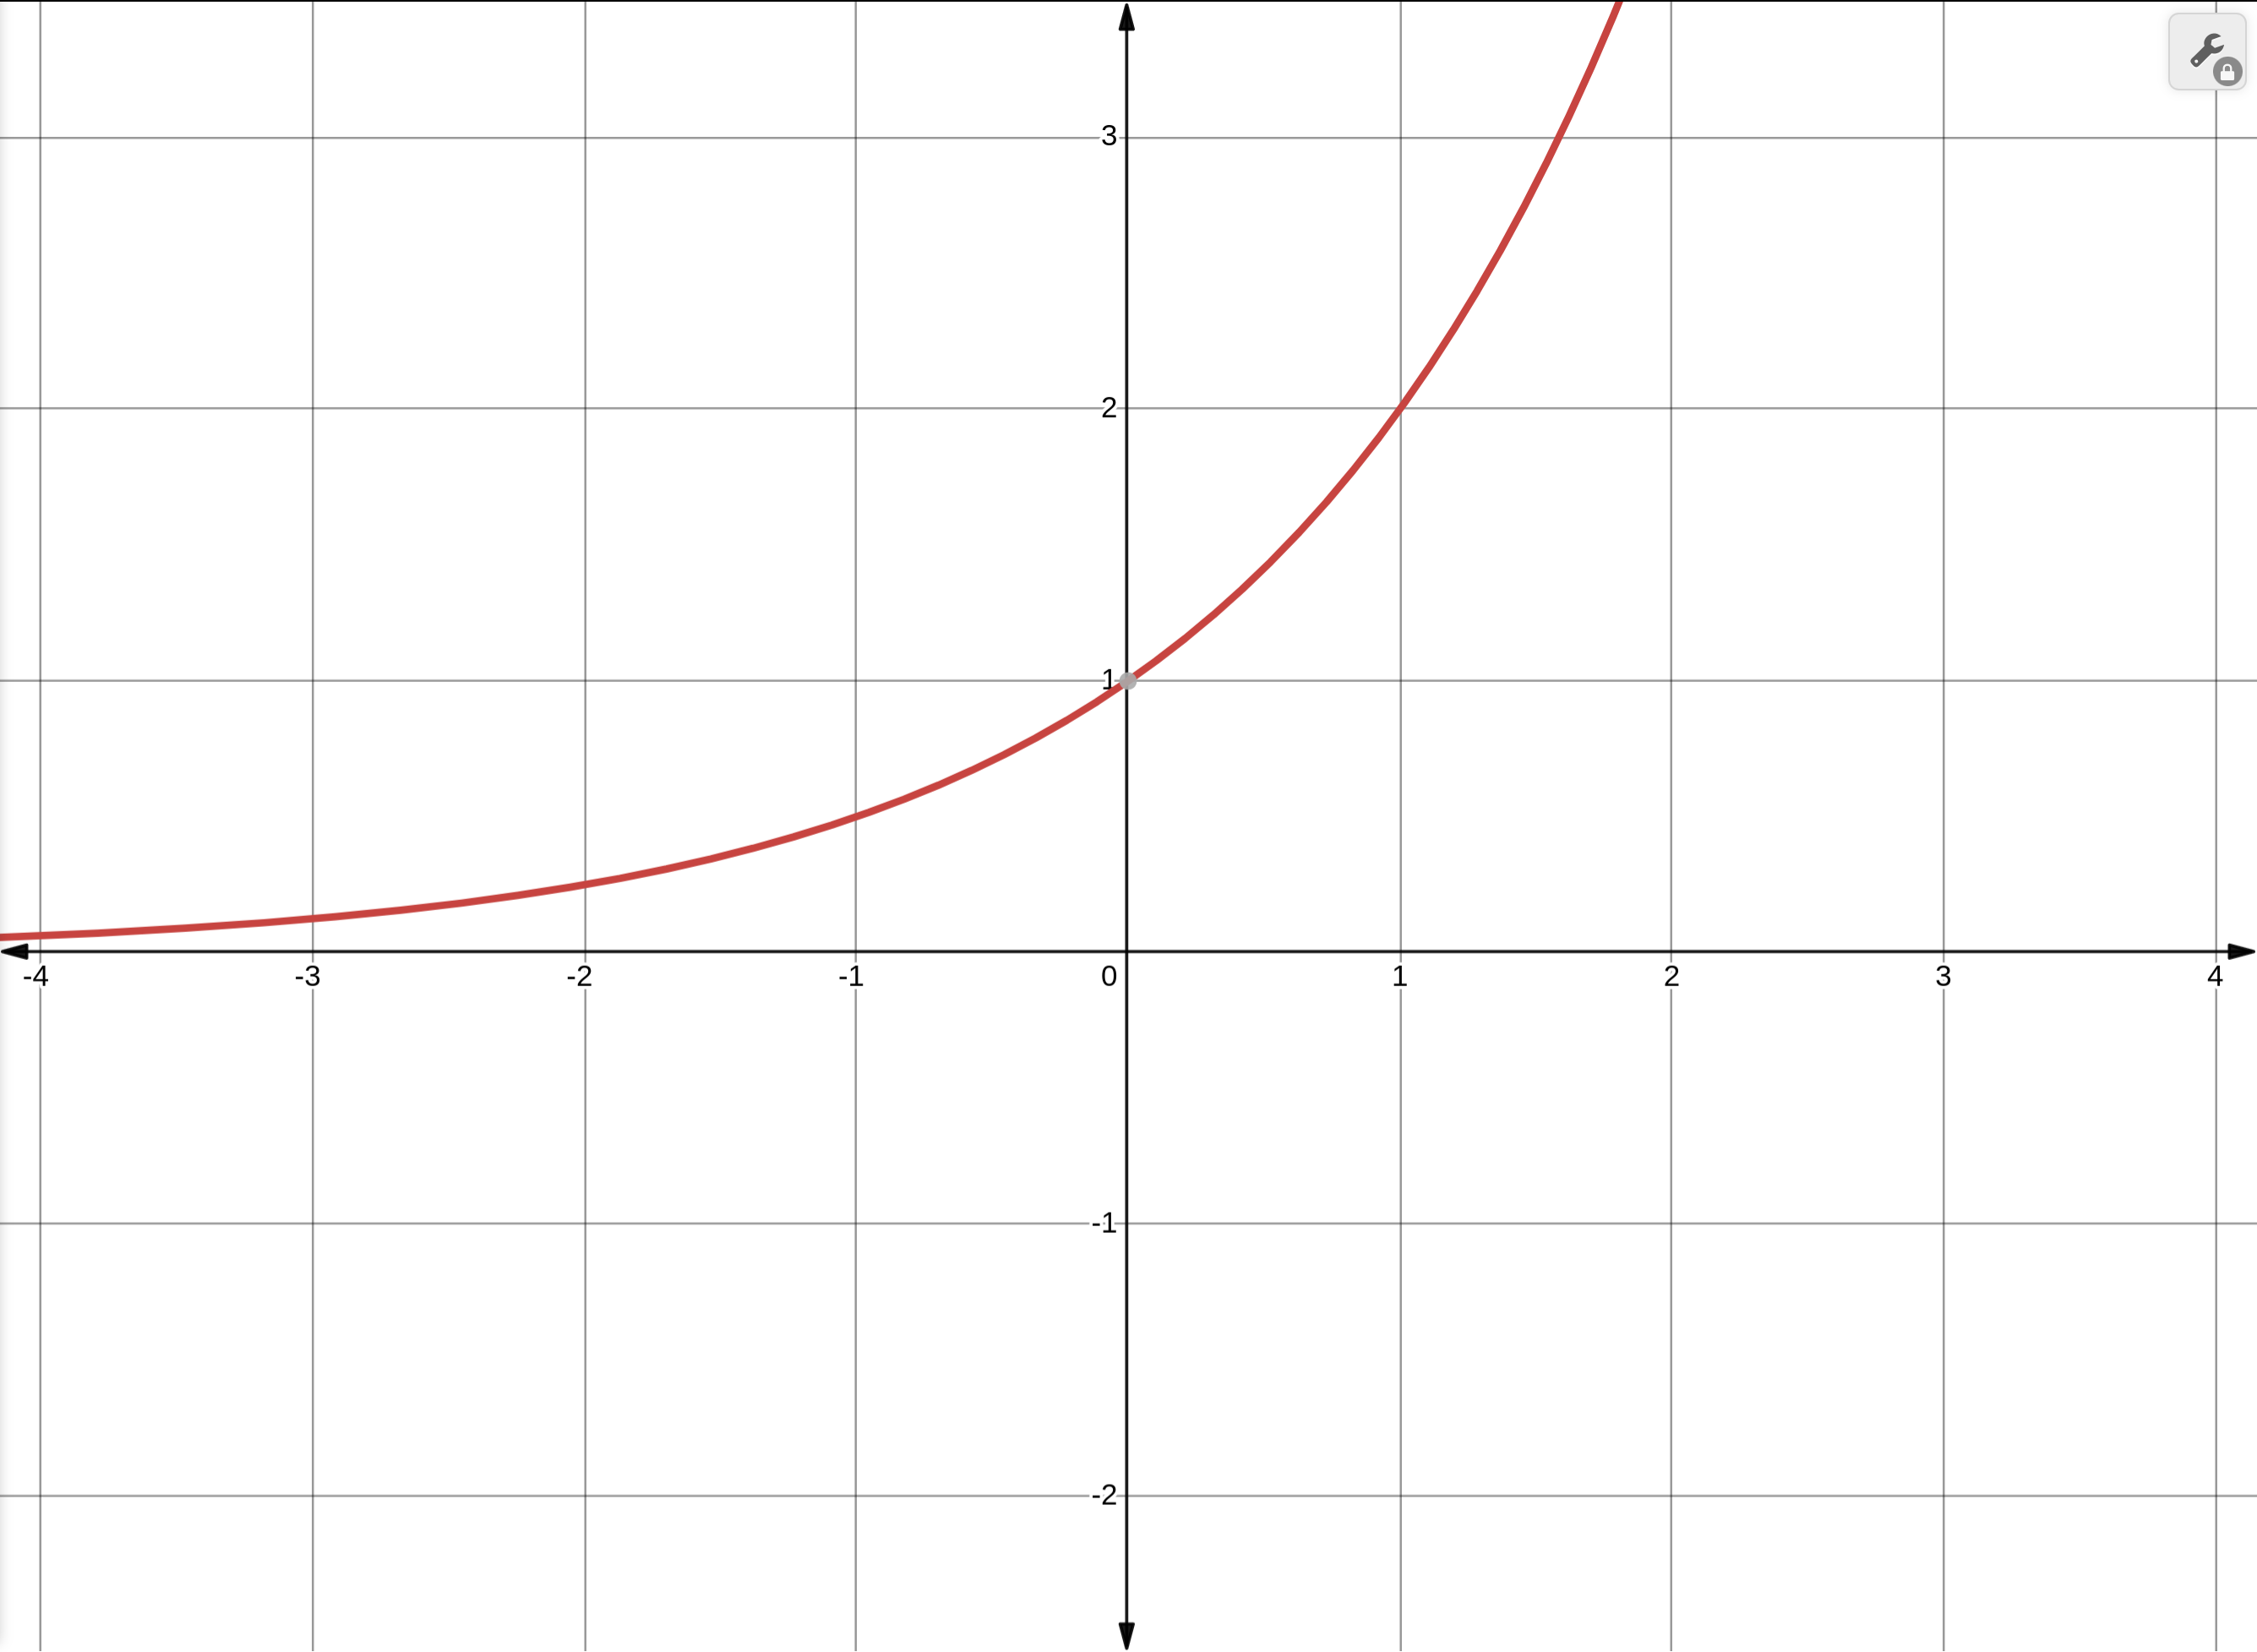
\includegraphics[scale=0.15]{"./fig/exp_1.png"}
\end{figure}
\subsection*{Graph of \(a^{x}\) when \(0<a<1\)}

\begin{figure}[H]
  \centering
  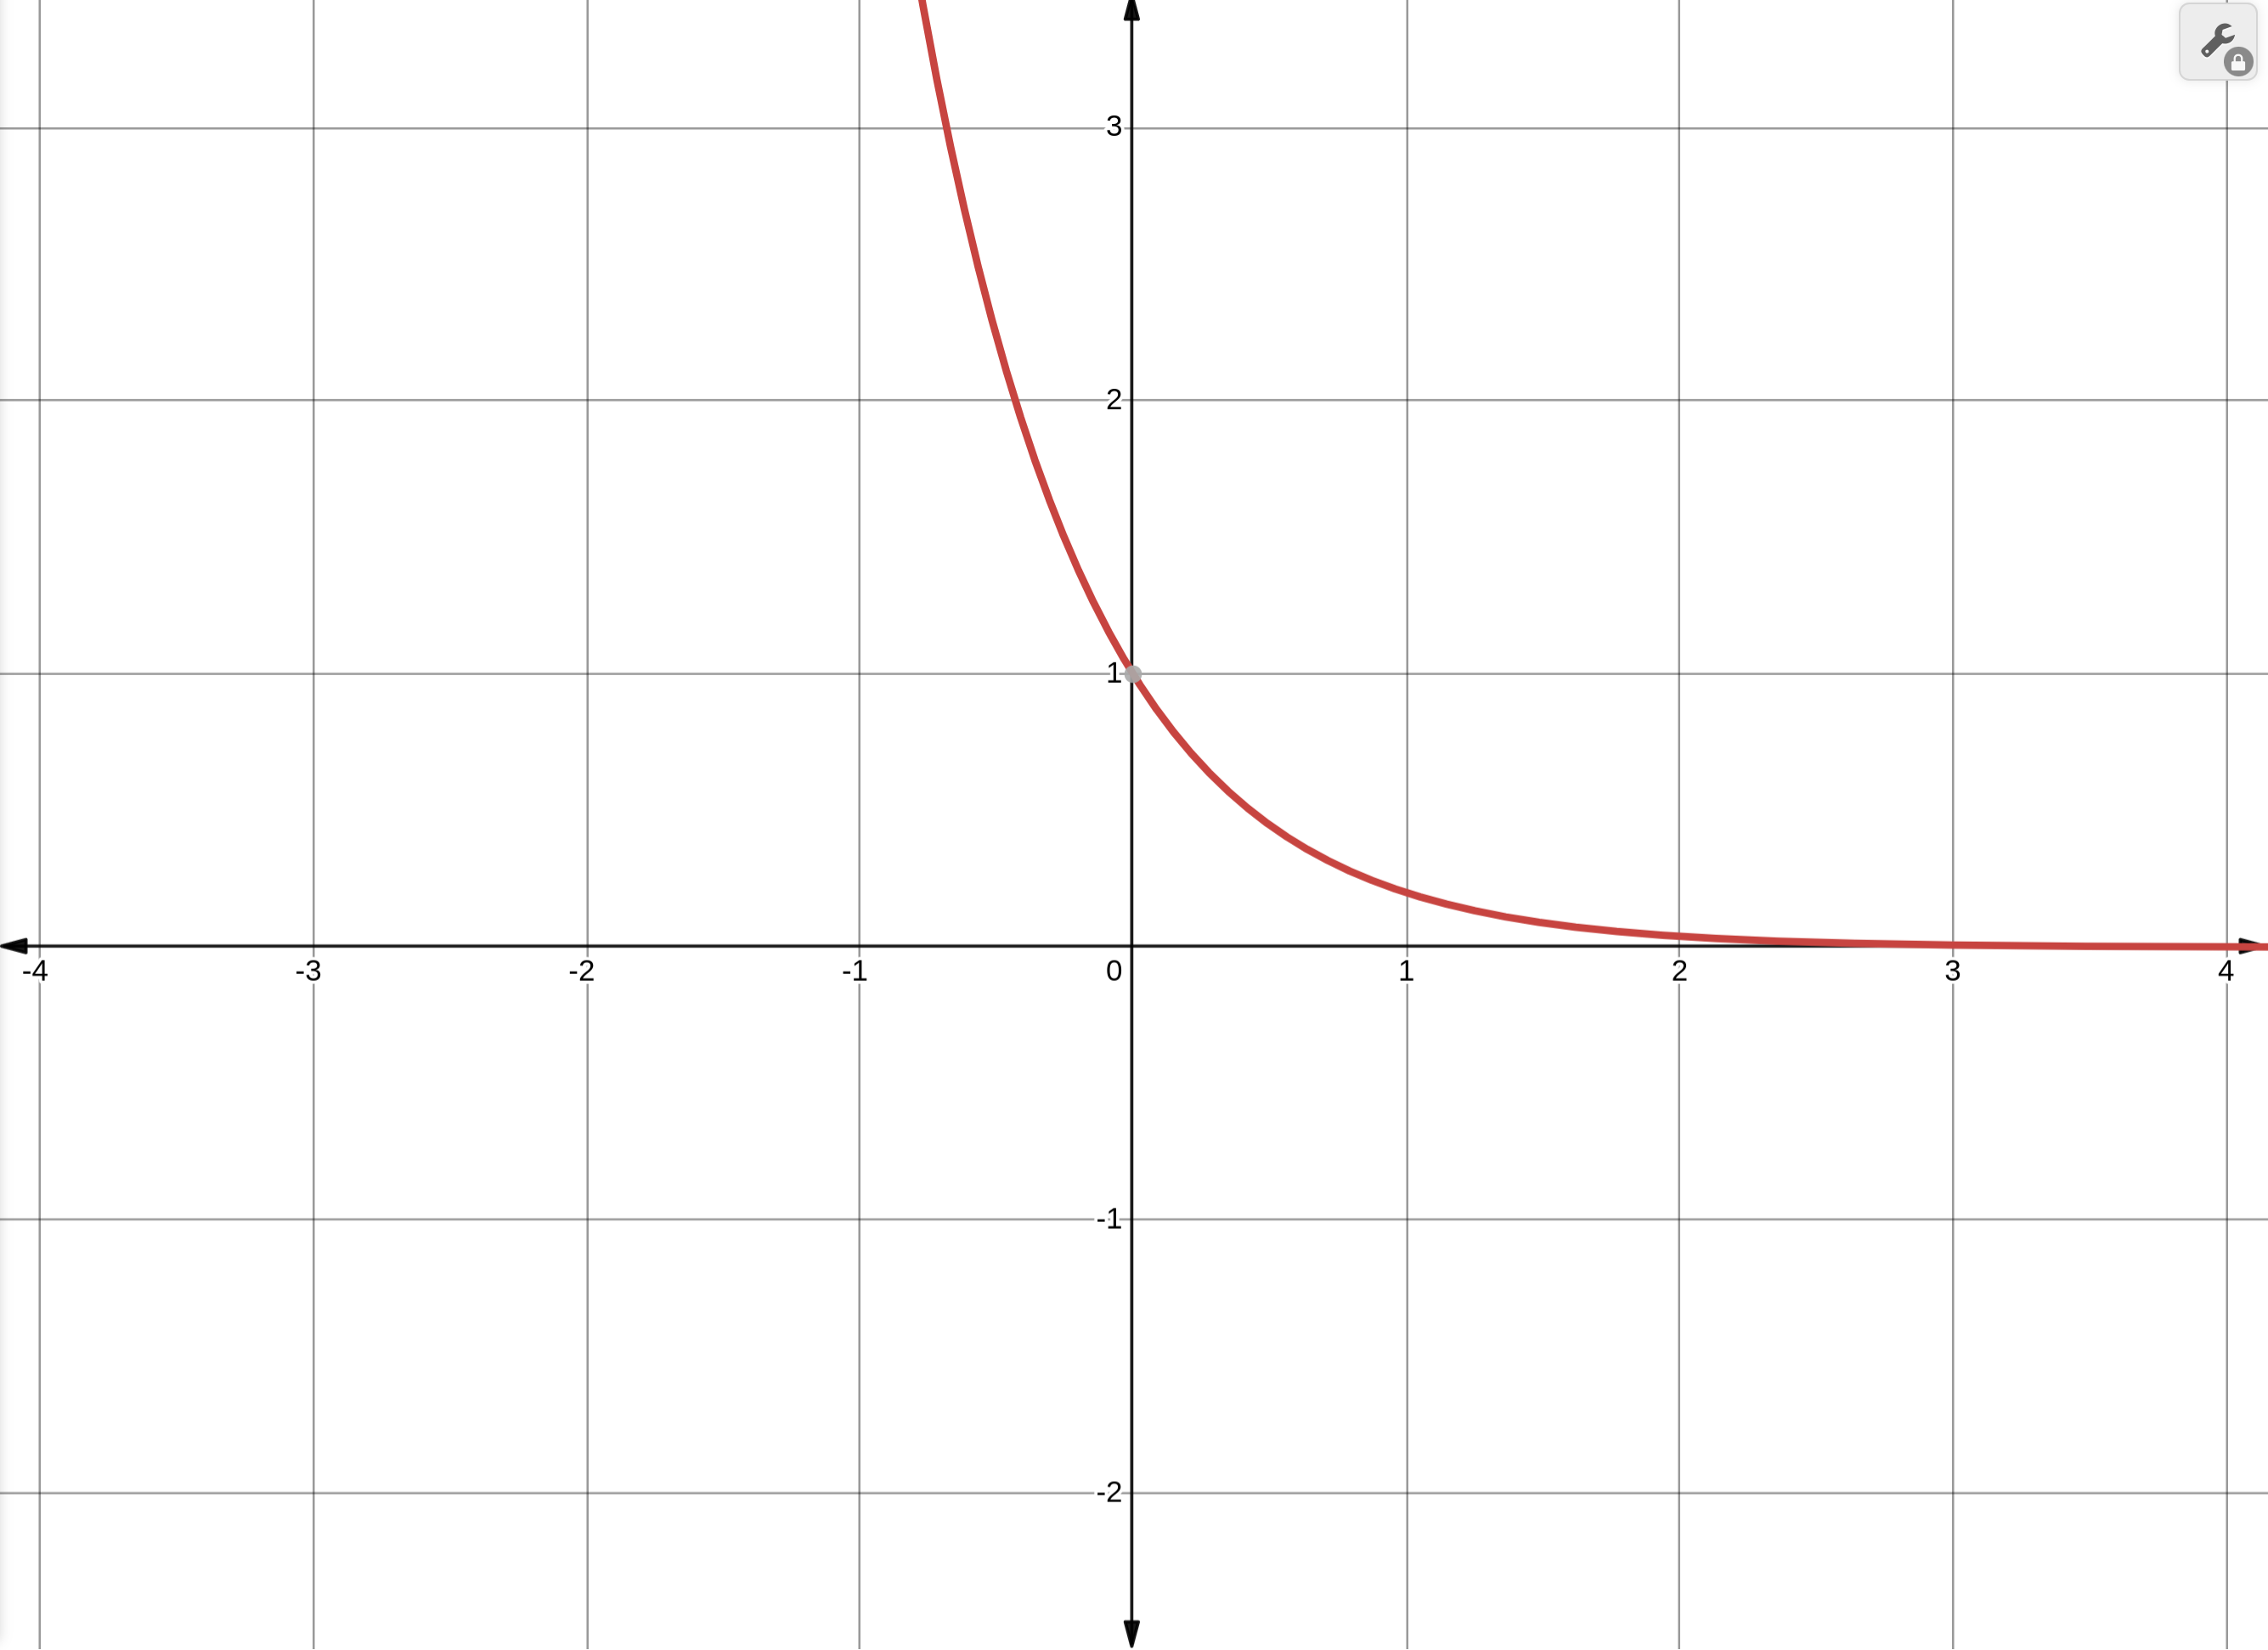
\includegraphics[scale=0.15]{"./fig/exp_2.png"}
\end{figure}

\begin{example}
  Plot the graph of \( f\left(x\right)\ =\ 6-5^{-x}\).
\begin{itemize}
\item Step 1. Plot \( 5^{-x} \) or $ \left( \frac{1}{5} \right)^{x} (black)$
\item Step 2.  Reflect  \( 5^{-x} \) to obtain \( -5^{-x} \) (blue)
\item Step 3.  Vertically translate  \( -5^{-x} \) to obtain \( 6-5^{-x} \) (green)
\end{itemize}

\begin{figure}[H]
  \centering
  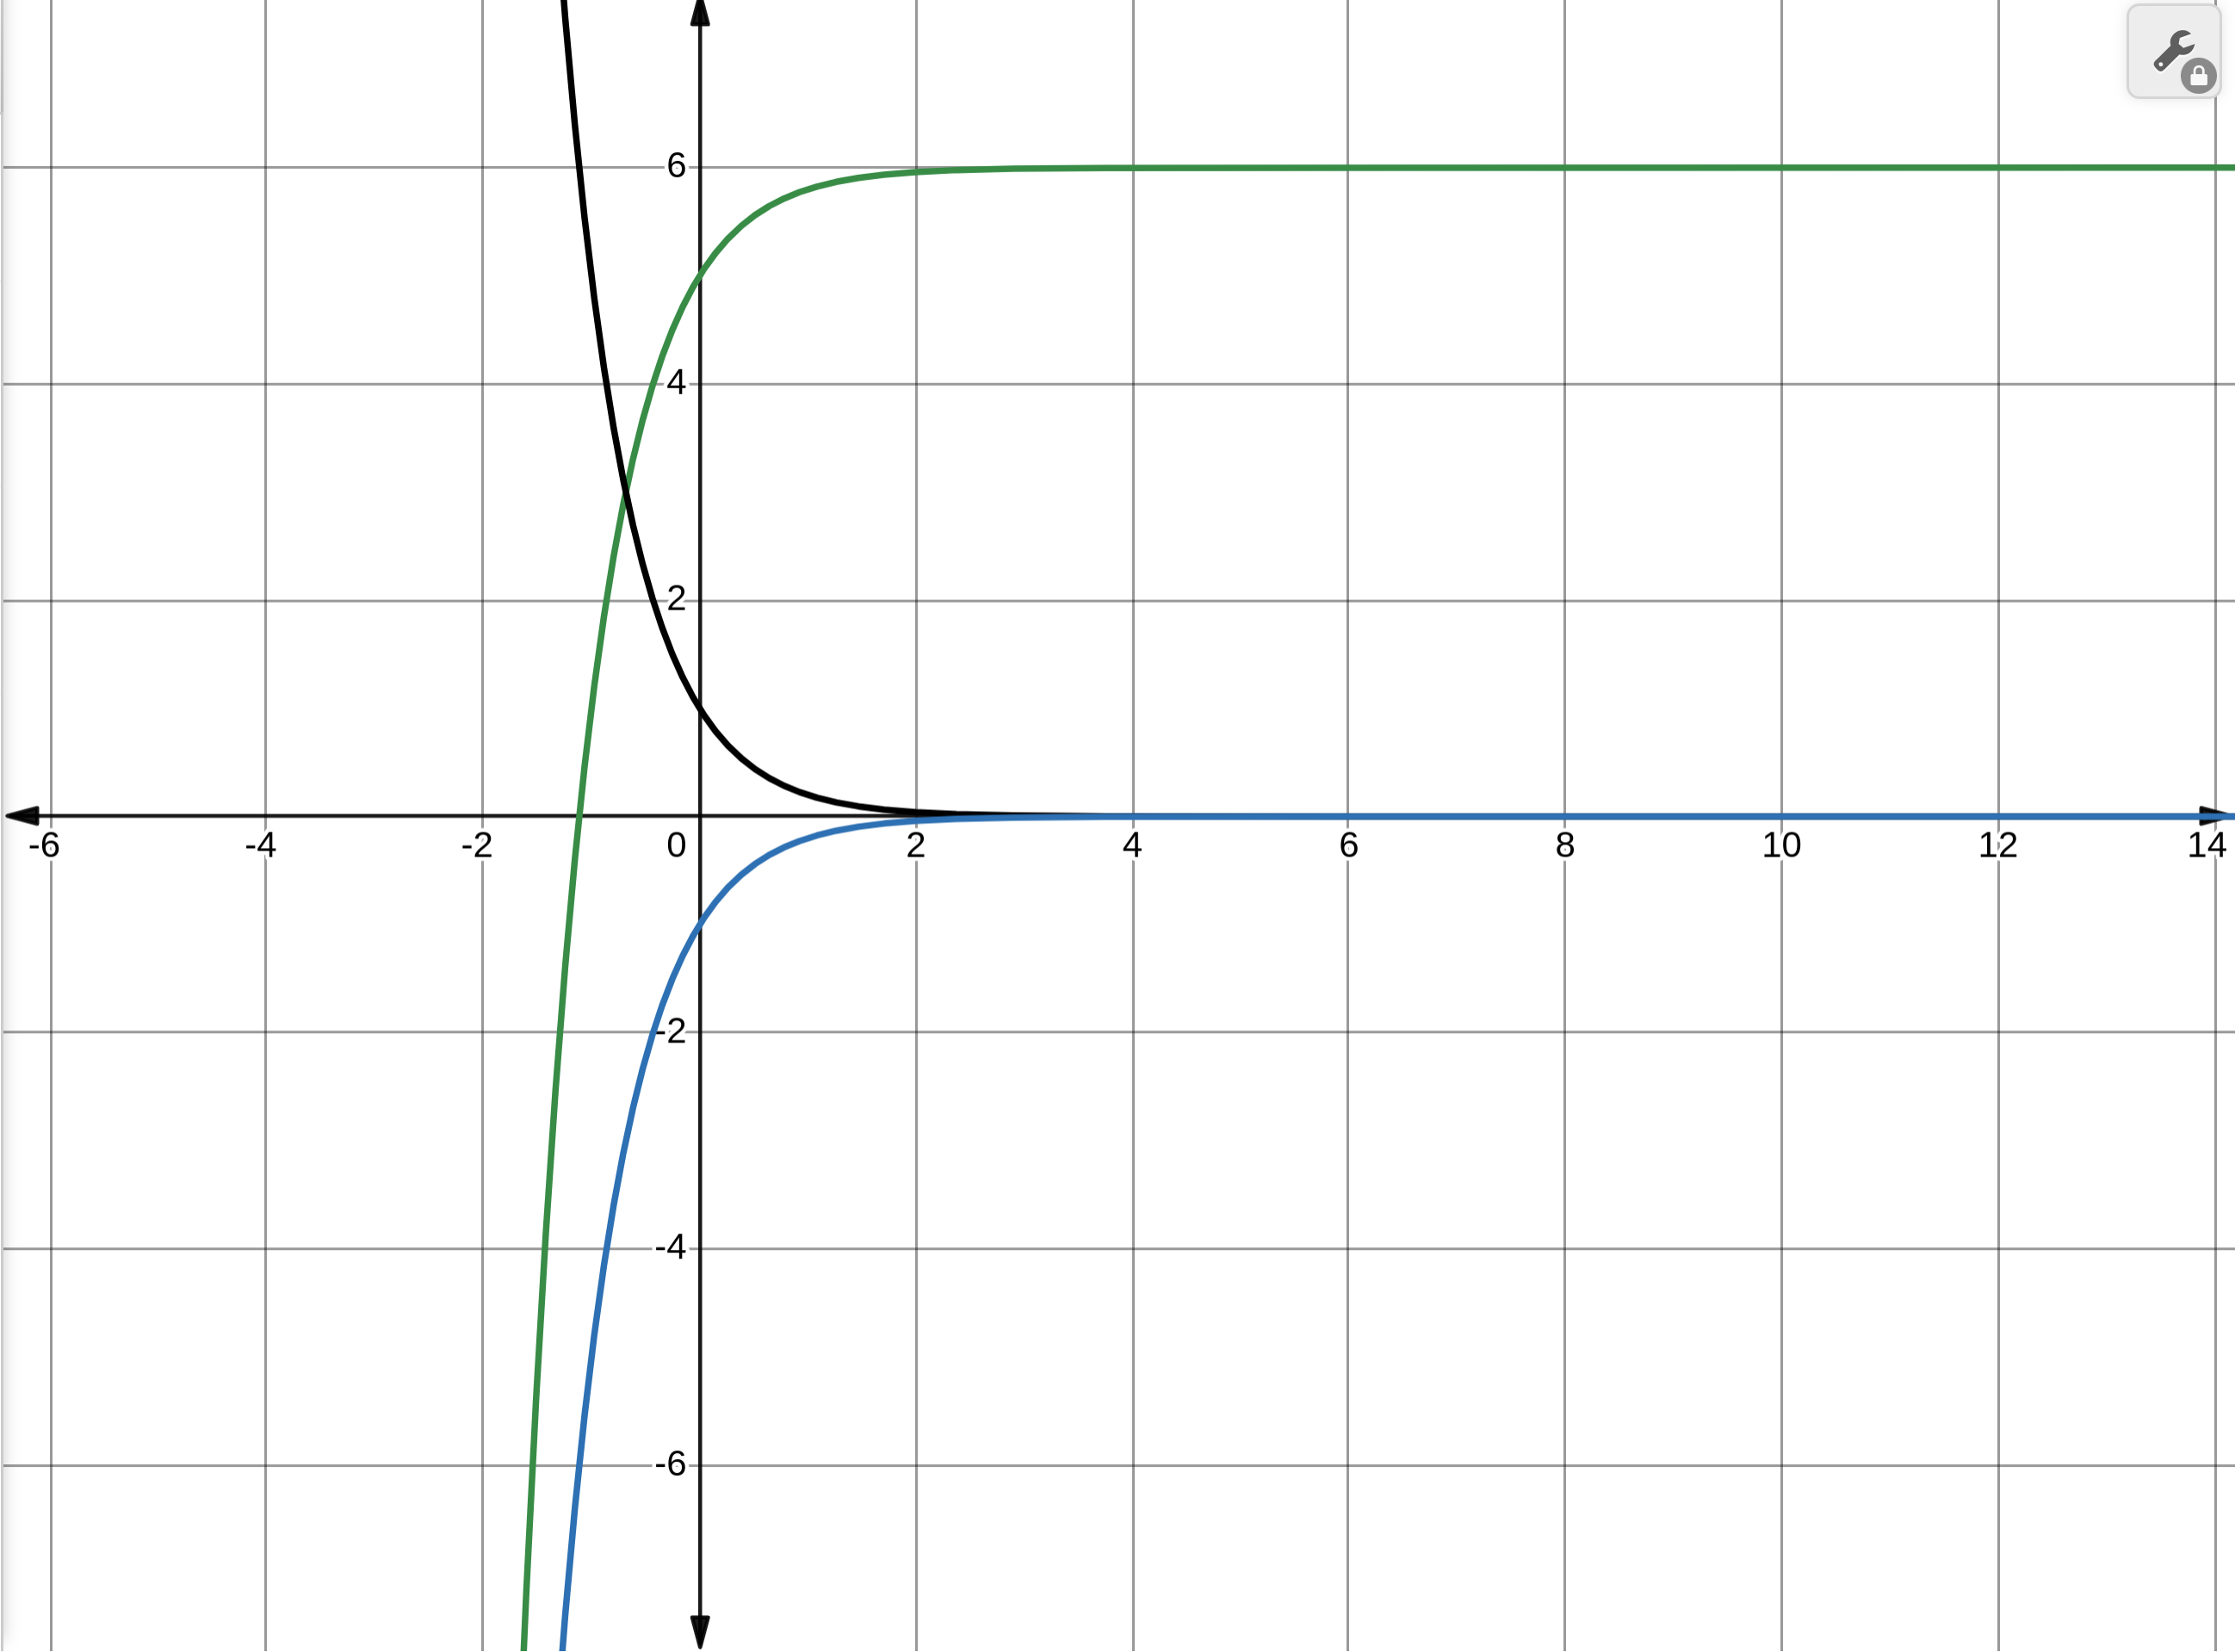
\includegraphics[scale=0.15]{"./fig/exp_tr.png"}
\end{figure}
\end{example}


\subsection{Solving Exponential Equations}

\begin{example} 

  Solve \(7^{x} = 343 \) for $x$

  Since \(7^{x} = 7^{3} \), therefor $x=3$


\end{example}


\begin{example}
  Solve \(64^{3x-1} = 16^{2x+3}\) for \(x\).
  
  Since \(64 = 2^6\) and \(16 = 2^4\), therefore
  
  \[
  \left( 2^6 \right)^{3x-1} = \left( 2^4 \right)^{2x+3}
  \]
  \[
  2^{6(3x-1)} = 2^{4(2x+3)}
  \]
  
 and
  
  \(6(3x-1) = 4(2x+3) \)
  or
  \(18x - 6 = 8x + 12 \)
  
  which results in 
  \(18x - 8x = 12 + 6 \)

   and gives us 
   \(x = \frac{18}{10} = \frac{9}{5} \)
  


\end{example}

\section{Logarithmic Functions}

We can express logarithmic equations in exponential form as follows:

\[
2^4 = 16 \quad \text{is equivalent to} \quad 4 = \log_2 16
\]
\[
3^2 = 9 \quad \text{is equivalent to} \quad 2 = \log_3 9
\]
\[
5^6 = 625 \quad \text{is equivalent to} \quad 6 = \log_5 625
\]
\[
10^x = 1000 \quad \text{is equivalent to} \quad ?
\]
\[
10^x = 15 \quad \text{is equivalent to} \quad ?
\]
\begin{definition}
[Logarithm]
A logarithm is the inverse operation of exponentiation. If we have an equation of the form:

\[
a^x = b
\]

then the logarithm of \( b \) with base \( a \) is defined as:

\[
\log_a b = x
\]
\end{definition}
This means that the logarithm of \( b \) with base \( a \) is the exponent \( x \) to which \( a \) must be raised to obtain \( b \).


\begin{itemize}
    \item The base \( a \) of a logarithm is a positive real number (except 1), and it determines the base of the exponential function.
    \item The argument \( b \) is the value for which we are finding the logarithm.
    \item The logarithm \( \log_a b \) gives the exponent to which the base \( a \) must be raised to equal \( b \).
\end{itemize}

\begin{example}
Solving a Basic Logarithmic Equation:

\[
\log_2 8 = x
\]

This asks: "To what power must 2 be raised to give 8?" We know that:

\[
2^3 = 8
\]

Thus:

\[
\log_2 8 = 3
\]

\end{example}

\begin{example}
 Converting Between Exponential and Logarithmic Form

The equation \( 10^x = 1000 \) can be written in logarithmic form as:

\[
\log_{10} 1000 = x
\]

Since \( 10^3 = 1000 \), we find that:

\[
\log_{10} 1000 = 3
\]

\end{example}


\begin{example}
Solving for \( x \) in a Logarithmic Equation
\end{example}

Solve the equation:

\[
\log_5 x = 3
\]

This means that \( 5^3 = x \), and solving for \( x \):

\[
x = 5^3 = 125
\]

Thus, the solution is \( x = 125 \).

\subsection{Properties of Logarithms}

Logarithms have several important properties that can help simplify calculations:

\begin{itemize}
 \item
\[
 \log_{a}1 = 0
\]

 \item
\[
 \log_{a}a = 1
\]
\item \textbf{Product Rule}
\[
\log_a (xy) = \log_a x + \log_a y
\]
\item \textbf{Quotient Rule}
\[
\log_a \left( \frac{x}{y} \right) = \log_a x - \log_a y
\]
\item \textbf{Power Rule}
\[
\log_a (x^n) = n \log_a x
\]
\item \textbf{Change of Base Formula}
\[
\log_a b = \frac{\log_c b}{\log_c a}
\]
\end{itemize}

\begin{example}
Change of Base Formula:
Using the change of base formula, we can compute \( \log_2 8 \) using base 10 logarithms:

\[
\log_2 8 = \frac{\log_{10} 8}{\log_{10} 2}
\]

\end{example}

\subsection{Common Logarithms and Natural Logarithms}

There are two special types of logarithms that are commonly used:

\subsection*{Common Logarithm}

The common logarithm has base 10 and is usually written as \( \log x \) (without specifying the base):

\[
\log x = \log_{10} x
\]

\subsection*{Natural Logarithm}

The natural logarithm has base \( e \) (where \( e \approx 2.718 \)) and is usually written as \( \ln x \):

\[
\ln x = \log_e x
\]

For example:

\[
\ln e = 1
\]

% \begin{example}
%   Use the properties of logarithms to write the expression as a sum,
%   difference, or product of simpler logarithms.
%   \begin{itemize}
%   \item $\log_{4}\sqrt{5x}$
%   \item $\log_{2} \left(\frac{4x}{5y} \right)$
%   \item $\log_{4}\sqrt{5x}$
%   \item $\ln\left (\frac{\sqrt{5x}}{\sqrt[3]{4}} \right)$ %cube root in last part
%   % \item $\log_{4}\sqrt{5x}$
%   \end{itemize}
% \end{example}

% \begin{example}
%   Solve the equation for $x$.
%   \begin{itemize}
%   \item $\log_{x} 625 = 4$ 
%   \item $\log_{4} (x+1) - \log_{4}(x-1)  = 1$ 
%   \item $\ln x + \ln 3x = 5 $
%   \item $e^{x+1} = 18$ 
%   \end{itemize}
% \end{example}

% \subsection{Applicatons}
% - Applications, Word Problems

%%% Local Variables:
%%% mode: LaTeX
%%% TeX-master: t
%%% End:

\begin{example}
  Use the properties of logarithms to write the expression as a sum,
  difference, or product of simpler logarithms.
  \begin{enumerate}
  \item $\log_{4}\sqrt{5x}$
  \item $\log_{2} \left(\frac{4x}{5y} \right)$
  \item $\log_{4}\sqrt{5x}$
  \item $\ln\left (\frac{\sqrt{5x}}{\sqrt[3]{4}} \right)$ %cube root in last part
  % \item $\log_{4}\sqrt{5x}$
  \end{enumerate}
\end{example}

\textbf{Solution:}
\begin{enumerate}
\item Using power rule we get
  \[
  \log_4 \sqrt{5x} = \log_4 (5x)^{1/2} = \frac{1}{2} \log_4 (5x)
  \]
  Since
  \[
   \log_4 (5x) =   \log_4 5 + \log_4 x 
  \]
  therefore
  \[
  \log_4 \sqrt{5x} = \frac{1}{2} \log_4 5 + \frac{1}{2} \log_4 x
\]

\item 
  \[
  \log_2 \left( \frac{4x}{5y} \right) = \log_2 (4x) - \log_2 (5y)
  \]
  since,
  \[
  \log_2 (4x) = \log_2 4 + \log_2 x
  \]
  and 
  \[
  \log_2 (5y) = \log_2 5 + \log_2 y
  \]
  therefore:
  \[
  \log_2 \left( \frac{4x}{5y} \right)=\log_2 4 + \log_2 x - (\log_2 5 + \log_2 y)
  \]
  Since \(\log_2 4 = \log_2 2^{2} = 2 \log_2 2 = 2\), the final expression is:
  \[
  \log_2 \left( \frac{4x}{5y} \right)=2 - \log_2 5 + \log_2 x - \log_2 y
  \]
\item Try yourself!
\item Try yourself!
\end{enumerate}



\begin{example}
  Solve the equation for $x$.
  \begin{enumerate}
  \item $\log_{x} 625 = 4$ 
  \item $\log_{4} (x+1) - \log_{4}(x-1)  = 1$ 
  \item $\ln x + \ln 3x = 5 $
  \item $e^{x+1} = 18$ 
  \end{enumerate}
\end{example}

\subsection{Applicatons}

\begin{example}
The census bureau for a large country has reported that the country is becoming more diverse. The projected population (in millions) of a certain minority is modeled by the exponential function
\[
h(t) = 37.67 \times (1.023)^t \quad \text{where} \quad 0 \leq t \leq 50.
\]
for the years 2000 to 2050.
Estimate in what year the minority's population will double the 2005 population of 42.21 million. 

\end{example}

\textbf{Solution}
We are given the population model:
\[
h(t) = 37.67 \times (1.023)^t
\]
and the population in 2005 is 42.21 million, we can verify this by.
\[
h(5) = 37.67 \times (1.023)^{5} \approx 42.21
\]
We need to find the year when the population doubles 
\(
2 \times 42.21 = 84.42 \text{ million}.
\)
Therefore
\[
84.42 = 37.67 \times (1.023)^t.
\]
and  Solve for \( t \)
\[
\frac{84.42}{37.67} = (1.023)^t,
\]
\[
2.24 = (1.023)^t.
\]

Take the natural logarithm (or any logarithm) of both sides, we get
\[
\ln(2.24) = t \ln(1.023).
\]

therefore:
\[
t = \frac{\ln(2.24)}{\ln(1.023)} \approx 
 0.8047, \quad \ln(1.023) \approx 0.0227,
\]
we get:
\[
t \approx \frac{0.8047}{0.0227} \approx 35.44.
\]

Thus, the population will double in approximately the year 2035.

\begin{example}
Find the present value of a deposit of \$40,000 at an interest rate of 4.1\% compounded continuously for 10 years.
\end{example}

\textbf{Solution}
The formula for the present value \( P \) when the amount \( A \) is compounded continuously is given by:
\[
A = P e^{rt}
\]
where \( r \) is the interest rate (4.1\% or 0.041).

We are given \( A = 40,000 \), \( r = 0.041 \), and  \( t = 10 \). 

\[
40,000 = P e^{0.041 \times 10}
\]
\[
40,000 = P e^{0.41}
\]

\[
P = \frac{40,000}{e^{0.41}}.
\]

\[
P \approx \frac{40,000}{1.506} \approx 26,546.01.
\]
